\newcommand{\DoNotLoadEpstopdf}{}
\documentclass[11pt]{article}
\usepackage[margin=1.05in]{geometry}
\usepackage[T1]{fontenc}
\usepackage{lmodern}
\input{glyphtounicode-cmex}
\pdfgentounicode=1
\usepackage{amsmath,amssymb,amsthm,mathtools,mathrsfs}
\usepackage{microtype}
\usepackage{booktabs,array}
\usepackage{tikz,flafter,float}
\usepackage[colorlinks=true,linkcolor=blue,citecolor=blue,urlcolor=blue]{hyperref}
\hypersetup{
 pdftitle={Contact Fano manifolds and the LeBrun–Salamon conjecture},
 pdfauthor={OpenAI},
 pdfsubject={Contact Fano classification and positive quaternionic-Kahler geometry}
}
\setlength{\emergencystretch}{1.5em}
\newtheorem{theorem}{Theorem}[section]
\newtheorem{proposition}[theorem]{Proposition}
\newtheorem{lemma}[theorem]{Lemma}
\newtheorem{corollary}[theorem]{Corollary}
\newtheorem{claim}[theorem]{Claim}
\theoremstyle{definition}
\newtheorem{definition}[theorem]{Definition}
\theoremstyle{remark}
\newtheorem{remark}[theorem]{Remark}
\numberwithin{equation}{section}
\newcommand{\CC}{\mathbb C}
\newcommand{\ZZ}{\mathbb Z}
\newcommand{\PP}{\mathbb P}
\newcommand{\OO}{\mathcal O}
\newcommand{\stacksTag}[1]{\href{https://stacks.math.columbia.edu/tag/#1}{\texttt{#1}}}
\DeclareMathOperator{\Pic}{Pic}
\DeclareMathOperator{\Hom}{Hom}
\DeclareMathOperator{\Aut}{Aut}
\DeclareMathOperator{\Spec}{Spec}
\DeclareMathOperator{\Proj}{Proj}
\DeclareMathOperator{\Tot}{Tot}
\DeclareMathOperator{\Lie}{Lie}
\DeclareMathOperator{\rank}{rank}
\DeclareMathOperator{\codim}{codim}
\DeclareMathOperator{\coker}{coker}
\DeclareMathOperator{\im}{im}
\DeclareMathOperator{\id}{id}
\DeclareMathOperator{\ad}{ad}
\DeclareMathOperator{\End}{End}
\DeclareMathOperator{\Sym}{Sym}
\DeclareMathOperator{\PGL}{PGL}
\DeclareMathOperator{\GL}{GL}
\DeclareMathOperator{\SL}{SL}
\DeclareMathOperator{\Sp}{Sp}
\DeclareMathOperator{\Rm}{Rm}
\title{Contact Fano manifolds and the\\ LeBrun--Salamon conjecture}
\author{OpenAI}
\date{September 23, 2026}
\begin{document}
\maketitle
\begin{abstract}
We resolve the contact-Fano homogeneity conjecture and the Riemannian
LeBrun--Salamon conjecture positively. Every smooth connected complex
projective contact Fano manifold of complex dimension at least three,
with its given contact distribution, is contact-isomorphic to the
adjoint variety of a simple complex Lie algebra. Consequently, every
closed connected smooth positive quaternionic-K\"ahler manifold of real
dimension $4m\geq8$ is homothetic to a compact symmetric Wolf space.
\end{abstract}
\section{Introduction}\label{sec:introduction}

Let $X$ be a smooth connected complex projective variety of dimension
$2n+1$, where $n\geq1$. A \emph{contact structure} on $X$ is an exact
sequence of algebraic vector bundles
\begin{equation}\label{intro:contact-sequence}
 0\longrightarrow F\longrightarrow T_X
 \xrightarrow{\ \theta\ }L\longrightarrow0,
\end{equation}
with $L$ a line bundle, such that the Levi pairing
\[
 F\otimes F\longrightarrow L,
 \qquad (v,w)\longmapsto\theta([v,w])
\]
is everywhere nondegenerate. In a local frame of $L$, write $\alpha$
for the scalar one-form representing $\theta$. The condition is
equivalent to $\alpha\wedge(d\alpha)^n$ being nowhere zero. We call
$(X,F)$ a \emph{contact Fano manifold} if $-K_X$ is ample.

For a simple complex Lie algebra $\mathfrak g$, let
$\mathcal O_{\min}(\mathfrak g)$ be its nonzero nilpotent adjoint orbit
of smallest dimension, and put
\[
 Y_{\mathfrak g}=\PP(\mathcal O_{\min}(\mathfrak g)).
\]
This is the unique closed adjoint orbit in $\PP(\mathfrak g)$. Its
canonical contact structure is obtained by projectivizing the
Kirillov--Kostant--Souriau symplectic cone.

\begin{theorem}\label{thm:main}
Let $(X,F)$ be a smooth connected complex projective contact Fano
manifold of dimension $2n+1$, with $n\geq1$, and let $L=T_X/F$.
There exist a finite-dimensional simple complex Lie algebra
$\mathfrak g$ and an algebraic isomorphism
\[
 \varphi:X\xrightarrow{\ \sim\ }Y_{\mathfrak g}
\]
whose differential carries the given distribution $F$ to the canonical
contact distribution on $Y_{\mathfrak g}$. Moreover,
\[
 L\simeq\varphi^*\bigl(\OO_{\PP(\mathfrak g)}(1)|_{Y_{\mathfrak g}}\bigr).
\]
\end{theorem}

Throughout the paper, $\PP(E)$ parametrizes lines in $E$, with
tautological subbundle $\OO_{\PP(E)}(-1)$. The two models separated
by the Picard reduction are
\[
 \begin{array}{c|c|c}
 X&L&\mathfrak g\\ \hline
 \PP^{2n+1}&\OO(2)&\mathfrak{sp}_{2n+2}(\CC)\\[2pt]
 \PP(T^*\PP^{n+1})&\OO(1,1)|_X&\mathfrak{sl}_{n+2}(\CC).
 \end{array}
\]
In the second row, $X$ is the incidence divisor of points and
hyperplanes in $\PP^{n+1}\times(\PP^{n+1})^*$. In the first, the
adjoint embedding is the quadratic Veronese embedding, so its
hyperplane bundle is $\OO(2)$. The proof then treats the remaining
case $\Pic(X)=\ZZ[L]$.

Two consequences will be proved after the classification in
Section~\ref{hom:section}.

\begin{corollary}[K\"ahler--Einstein existence]\label{thm:contact-fano-ke}
Let $(X,F)$ be a smooth connected complex projective contact Fano
manifold of complex dimension $2n+1$, where $n\geq1$. Then $X$ admits a
K\"ahler--Einstein metric of positive scalar curvature for its given
complex structure.
\end{corollary}

For projective contact manifolds without a Fano hypothesis, the
results of Demailly and Kebekus--Peternell--Sommese--Wi\'sniewski
provide a reduction to which Theorem~\ref{thm:main} applies.

\begin{corollary}[Projective contact manifolds]\label{thm:projective-contact}
Let $(X,F)$ be a smooth connected complex projective contact manifold
of dimension $2n+1$, where $n\geq1$. Its second Betti number determines
the following alternatives.
\begin{enumerate}
\item If $b_2(X)=1$, then $(X,F)$ is contact-isomorphic to the adjoint
variety $Y_{\mathfrak g}$, with its canonical contact distribution, for
a simple complex Lie algebra $\mathfrak g$.
\item If $b_2(X)\geq2$, then there is a smooth connected complex
projective manifold $Z$ of dimension $n+1$ and a biholomorphism
\[
 X\simeq\PP(T^*Z).
\]
Here $\PP(T^*Z)$ parametrizes lines in cotangent spaces, equivalently
hyperplanes in tangent spaces. This assertion identifies the underlying
manifolds, without imposing compatibility with the given distribution $F$.
\end{enumerate}
Conversely, every adjoint variety of complex dimension $2n+1$ and every
projectivized cotangent bundle in the second alternative admits a contact
structure. Thus these are precisely the underlying manifolds of smooth
connected complex projective contact manifolds in these dimensions.
\end{corollary}

The Riemannian application concerns a smooth manifold of real
dimension $4m$, $m\geq2$, whose metric has holonomy contained in
$\Sp(m)\Sp(1)$ in its standard representation. Such a metric is
called \emph{quaternionic-K\"ahler}; \emph{positive} here means that
its scalar curvature is positive. The compact symmetric positive
quaternionic-K\"ahler spaces are the \emph{Wolf spaces}.

\begin{corollary}\label{thm:quaternionic}
Let $(M^{4m},g)$ be a closed connected smooth Riemannian manifold,
where $m\geq2$, with holonomy contained in $\Sp(m)\Sp(1)$ in the
standard representation and with positive scalar curvature. Then
\[
 \nabla\Rm_g=0.
\]
Moreover, $(M,g)$ is homothetic to a compact symmetric positive
quaternionic-K\"ahler Wolf space.
\end{corollary}

Theorem~\ref{thm:main} resolves the smooth contact-Fano homogeneity
conjecture positively. Corollary~\ref{thm:quaternionic} gives the
positive resolution of the Riemannian LeBrun--Salamon conjecture in
every real dimension $4m$ with $m\geq2$. The link is the positive
twistor construction: the twistor space is contact Fano, so the
general algebraic theorem applies to it. Simple connectivity of the
contact Fano twistor space and its $S^2$-bundle structure show that
the original manifold is simply connected. The metric is recovered
from the resulting complex twistor space in Section~\ref{tw:section}.

\subsection*{History and prior work}

The conjectural classification has two related settings.  Wolf's work
relates compact quaternionic symmetric spaces to homogeneous complex contact
spaces~\cite{Wolf1965}; the adjoint-variety description of their twistor
fibration is recalled in~\cite[Section~3.9, pp.~105--106]{LandsbergManivel2004}.
The twistor construction of Salamon, independently due to B\'erard-Bergery,
associates a contact Fano manifold to a closed connected positive
quaternionic-K\"ahler manifold~\cite{Salamon1982,LeBrun1995}.  LeBrun's converse characterizes the
contact Fano manifolds arising in this way by the existence of a
K\"ahler--Einstein metric~\cite[Theorem~A]{LeBrun1995}.  The finiteness and
rigidity program of LeBrun and Salamon~\cite{LeBrun1993,LeBrunSalamon1994}
provides the historical setting for the homogeneity conjecture.  The general
algebraic formulation, stated for example in
\cite[Conjecture~1.1]{Buczynski2010}, concerns every contact Fano manifold.

The projective-contact reduction has two ingredients. Kebekus,
Peternell, Sommese and Wi\'sniewski classify projective contact
manifolds with non-nef canonical bundle as either Fano with $b_2=1$
or projectivized cotangent bundles \cite[Theorem~1.1]{KPSW2000}.
Demailly's integrability theorem excludes pseudoeffectivity of the
canonical bundle of a compact K\"ahler contact manifold; his
Corollaries~3--4 give the reduction used in
Corollary~\ref{thm:projective-contact}
\cite[Corollaries~2--4]{Demailly2000}.
Within the Fano class, Mori's ample-tangent theorem and the
Kobayashi--Ochiai index theorem identify the incidence and
projective-space alternatives \cite{Mori1979,KO1973}. In the
remaining primitive case, Kebekus establishes the covering contact
lines and the spanning of their tangent directions
\cite{Kebekus2001}. For $n\geq2$, the corrected contact-line theorem gives a smooth,
possibly disconnected, Legendrian variety of directions
\cite[corrected version, Theorem~3.1 and Remark~3.2]{Buczynski2010}.
The case $n=1$ is treated directly in Section~\ref{lines:section}.
These results identify the geometric objects from which the
smoothing, tensor descent and diagonal arguments below begin.


Earlier low-dimensional classifications were obtained by Poon and Salamon
for compact positive quaternionic-K\"ahler manifolds in real dimension
eight~\cite{PoonSalamon1991}, and by Ye and Druel for contact Fano manifolds in
complex dimensions three and five, respectively
\cite{Ye1994,Druel1998}.
Several classification results impose additional geometric or
group-theoretic hypotheses.  Beauville's contact moment-map approach gives adjoint
classification when the contact linear-system map is generically finite and
the contact automorphism group is reductive~\cite[Theorem~0.1]{Beauville1998}.
Yasukura proves adjoint classification for compact connected complex
contact manifolds whose contact line bundle defines a holomorphic
immersion~\cite[Theorem~1.1]{Yasukura2023v12}. The first-jet generation
obtained below supplies such an immersion; we give the resulting
contact moment-map classification directly.
Buczy\'nski and Wi\'sniewski classify the closed positive quaternionic-K\"ahler
manifolds in real dimensions twelve and sixteen, and the contact Fano
manifolds in complex dimensions three through nine with reductive automorphism
group~\cite[Theorems~1.1--1.2]{BW2022}.
Occhetta, Romano, Sol\'a Conde, and Wi\'sniewski prove the adjoint
classification in the primitive Picard case under reductivity and the rank
bound $r\geq\max\{2,(n-3)/2\}$ in complex dimension $2n+1$,
where $r$ is the rank of the contact automorphism group
\cite[Theorem~6.1]{OcchettaEtAl2021}.
On the Riemannian side, Brendle and Semmelmann establish symmetry for
compact positive quaternionic-K\"ahler manifolds of real dimension at least
eight under nonnegative sectional curvature
\cite[Corollary~2]{BrendleSemmelmann2025}.

The use of contact lines and two-line loci has substantial antecedents.
Buczy\'nski attributes the study of loci swept out by two contact lines to
Wi\'sniewski~\cite[Introduction]{Buczynski2010} and develops their divisors, duality, and
associated bilinear forms~\cite[Introduction and Theorem~1.3]{Buczynski2010}.
The Legendrian secant geometry of Landsberg and Manivel
\cite[Proposition~17(2) and its proof]{LandsbergManivel2007}
is used in Buczy\'nski's Proposition~3.5, which also records the
disjoint-join statement~\cite{Buczynski2010}.
Here a suitable pair of contact lines is smoothed, two vector lifts are
extended across the unmarked degree-two boundary, and their common contact
value descends to a symmetric tensor on the square.  Its diagonal jets
generate ordinary first jets of the contact line bundle at every point,
which yields transitivity of contact automorphisms.  The final jet criterion
also applies to compact complex contact manifolds satisfying its tensor
hypothesis, without a Fano assumption.

Kobayashi's preprint claims the Wolf-space classification for complete
locally irreducible positive quaternionic-K\"ahler manifolds of real
dimension at least eight
\cite[Theorem~5.3]{Kobayashi2008} and states K\"ahler--Einstein existence
for arbitrary contact Fano manifolds as a separate conjecture
\cite[Conjecture~1.3]{Kobayashi2008}. Corollary~\ref{thm:contact-fano-ke}
establishes this existence for the manifolds in Theorem~\ref{thm:main}.
Earlier versions of Yasukura's preprint asserted unrestricted contact-Fano
and quaternionic-K\"ahler classifications
\cite[Theorem~I and Corollary~II]{Yasukura2009v3},
\cite[Theorems~C--D and Corollary~E]{Yasukura2022v11}.
The author's later comments identify an error in Theorem~3.2(ii) of the
former version~\cite{Yasukura2009v4}, and identify Theorem~A and
Corollary~B of the latter version as false~\cite{Yasukura2023v12}.


\subsection*{The mechanism of the proof}

The \emph{contact degree} of a map $f:\PP^1\to X$ is
$\deg f^*L$. We call such a map a \emph{contact line} if its contact
degree is one and a \emph{conic} if its contact degree is two; these
terms impose no embedding assumption.

The objective is to produce enough global vector fields preserving
$F$ to span every tangent space. After the two explicit Picard
alternatives have been handled, we work with $\Pic(X)=\ZZ[L]$ and
construct a symmetric section
\begin{equation}\label{intro:global-section}
 B\in H^0(X\times X,L\boxtimes L),\qquad
 L\boxtimes L=\operatorname{pr}_1^*L\otimes\operatorname{pr}_2^*L,
\end{equation}
where $\operatorname{pr}_1,\operatorname{pr}_2$ are the projections
from $X\times X$. Near two coincident points the section vanishes
to second order, with leading term given by the square of the
contact form. This local behavior will force the global contact
fields to span. The construction has four stages.

First, at a general point choose two free contact lines, meaning
that their pulled-back tangent bundles are globally generated.
Their positive-degree tangent-bundle summands span $F_x$ and their tangent
vectors have nonzero Levi pairing. Their union can be smoothed
while its two outer values move. The key calculation concerns
the contrary, fixed-end problem: a first-order smoothing keeping
both values fixed would force the Levi pairing to vanish. The
fixed-end obstruction space is one-dimensional, so varying the
smoothing parameter supplies exactly the missing direction for
two-point evaluation. The resulting conic $g:\PP^1\to X$ is
\emph{very free}, meaning that every summand of $g^*T_X$ has
positive degree (Proposition~\ref{sm:very-free}). We keep all
nearby parametrized maps, not just a chosen one-parameter
smoothing, because the later diagonal calculation varies both
their values and their velocities.

Second, compactify these conics in the unmarked stable-map
space. Its universal-curve square parametrizes a source curve
together with two variable evaluation points. On a smooth source,
the coordinate-independent tensor
\[
 (z-w)^2\partial_z\otimes\partial_w
\]
gives two vector-valued sections, one retaining the tangent vector
in the first factor and one retaining it in the second. Applying
the contact form to both factors gives their common contact value.
The singular unmarked sources have exactly two degree-one
components. At a node of thickness $r$, the contact differential
vanishes to order at least $r$, canceling each possible pole of
the tensor. Both vector-valued sections consequently extend over
the proper family (Proposition~\ref{ext:moving-pair}).

Third, the common contact value descends from this proper family
to the section $B$ in \eqref{intro:global-section}. The two vector
lifts test contact lines in the two factors of $X\times X$.
On every proper integral component dominating a test line, the
relevant lift has constant projection to the trivial quotient of
the pulled-back tangent bundle. This forces every generic sheet
of the finite contact-value image to split over that line. A test
line meeting a hypothetical branch divisor transversely would
instead produce a sheet of degree greater than one. Purity and
simple connectedness then complete the descent
(Proposition~\ref{des:descent}).

Finally, on the full neighborhood of $g$ the section satisfies
\[
 B(h(z),h(w))=(z-w)^2\,
 \theta(h'(z))\otimes\theta(h'(w)).
\]
The available value and velocity variations make its constant
and linear diagonal terms vanish and identify the quadratic
symbol with $\theta^2$. Each of these intrinsic identities
extends from a nonempty open subset to all of $X$. Symmetry then
determines the cubic Taylor term in local coordinates and a line
frame. The quadratic and cubic terms imply that global sections
of $L$ generate first jets at every point. Contact Hamiltonians
therefore span every tangent space, giving contact transitivity
(Theorem~\ref{jet:criterion}). The contact moment map identifies
the resulting homogeneous manifold, with its given distribution,
with a simple adjoint variety (Proposition~\ref{hom:adjoint}).

Two parts of this mechanism have independent formulations:
contact-value descent from a proper family with the two vector
lifts, and the symmetric-jet criterion on a connected compact
complex contact manifold. The latter does not require projectivity
or Fano positivity. Global diagonal identities are what pass
from the initially general points to every point. After
transitivity is proved, Corollary~\ref{jet:good-curves} supplies
through every point in the primitive Picard case a conic transverse
to $F$ with $u^*F\simeq\OO(1)^{\oplus2n}$.

\subsection*{Conventions and organization}

All schemes, algebraic spaces and stacks are over $\CC$.
Curve families have their
scheme-theoretic fibers. ``General'' means outside a proper
Zariski-closed subset unless an analytic open set is explicitly
specified. For bundles $E_1,E_2$ on $X$, we similarly write
$E_1\boxtimes E_2=\operatorname{pr}_1^*E_1\otimes
\operatorname{pr}_2^*E_2$.

Section~\ref{red:section} proves the Picard reduction.
Section~\ref{lines:section} selects the pair of contact lines,
and Section~\ref{sm:section} smooths it to a very free conic.
Section~\ref{ext:section} extends the two moving-point tensors
over the unmarked boundary; Section~\ref{des:section} descends
their contact value. Section~\ref{jet:section} turns its diagonal
jets into contact transitivity, and Section~\ref{hom:section}
identifies the adjoint model and completes Theorem~\ref{thm:main}.
Section~\ref{tw:section} gives the twistor construction and
normalized metric recovery proving Corollary~\ref{thm:quaternionic}.

\section{The contact line and the Picard alternatives}
\label{red:section}

Let $X$ be a smooth connected complex projective contact Fano manifold
of dimension $d=2n+1$, where $n\geq1$, with contact sequence
\begin{equation}\label{red:contact}
0\longrightarrow F\longrightarrow T_X
\xrightarrow{\theta}L\longrightarrow0.
\end{equation}
In a local frame of $L$ we write $\alpha$ for $\theta$. With the Levi
convention in Section~\ref{sec:introduction}, local sections $v,w$ of
$F$ satisfy $d\alpha(v,w)=-\alpha([v,w])$.
The top exterior power of $d\alpha|_F$ is nowhere zero. Taking determinants gives
\begin{equation}\label{red:determinant}
\det F\simeq L^{\otimes n},\qquad
-K_X\simeq L^{\otimes(n+1)}.
\end{equation}
In particular $L$ is ample.

\begin{lemma}\label{red:simply-connected}
The manifold $X$ is simply connected, and its Picard group is a free
abelian group of finite rank, canonically isomorphic to $H^2(X,\ZZ)$.
\end{lemma}

\begin{proof}
We recall an argument that applies to every smooth complex Fano
manifold. Yau's prescribed-Ricci-form Theorem~\cite[Theorem~1]{Yau1977},
proved in~\cite{Yau1978}, says that
a real closed $(1,1)$-form representing $2\pi c_1(X)$ is the Ricci form
of a K\"ahler metric in any prescribed K\"ahler class. Ampleness of
$-K_X$ supplies a positive representative. For the resulting metric,
compactness gives a uniform positive lower bound for the Ricci tensor.
The Bonnet--Myers Theorem~\cite{Myers1941} makes the universal cover
$q:\widetilde X\to X$ compact, so $q$ has finite degree $r$.

The cover is holomorphic and unramified, and the lifted metric
is K\"ahler with positive Ricci tensor. In particular
$-K_{\widetilde X}=q^*(-K_X)$ is positive. Kodaira's projectivity
Theorem~\cite[Section~3, p.~316]{Kodaira1954} therefore makes the
compact manifold $\widetilde X$ projective. The graph of $q$ is a
closed analytic subvariety of the projective product
$\widetilde X\times X$, so GAGA makes $q$ algebraic
\cite[Proposition~15]{Serre1956}. It is proper with finite fibers, hence finite,
and its local analytic inverses show that it is \'etale.
Thus both manifolds and their finite covering are algebraic before
we apply projective vanishing and Riemann--Roch.

Kodaira vanishing~\cite{Kodaira1953}, applied to $\OO=K\otimes K^{-1}$, gives
$H^i(\widetilde X,\OO_{\widetilde X})=H^i(X,\OO_X)=0$ for $i>0$.
Both holomorphic Euler characteristics are one. Since
$T_{\widetilde X}=q^*T_X$, Hirzebruch--Riemann--Roch~\cite{Hirzebruch1954} gives
\[
1=\chi(\widetilde X,\OO_{\widetilde X})
 =\int_{\widetilde X}q^*\operatorname{td}(T_X)
 =r\,\chi(X,\OO_X)=r.
\]
Thus $X$ is simply connected. This argument prescribes a Ricci form;
it does not require the metric to be K\"ahler--Einstein.

The exponential sequence and the vanishings of $H^1(X,\OO_X)$ and
$H^2(X,\OO_X)$ identify the analytic Picard group with $H^2(X,\ZZ)$;
GAGA~\cite{Serre1956} identifies it with the algebraic Picard group. The cohomology
group is finitely generated. The universal coefficient sequence
has torsion term $\operatorname{Ext}^1(H_1(X,\ZZ),\ZZ)=0$, since
$H_1(X,\ZZ)=0$, and identifies $H^2(X,\ZZ)$ with a subgroup of a
finitely generated free abelian group. It is therefore free.
\end{proof}

\begin{proposition}\label{red:alternatives}
Either $\operatorname{Pic}(X)=\ZZ[L]$, or $(X,F)$ is contact-isomorphic
to one of the following standard contact manifolds:
\begin{enumerate}
\item the incidence variety
\[
I=\{(\ell,H)\in\PP^{n+1}\times(\PP^{n+1})^*: \ell\subset H\},
\qquad L=\OO_I(1,1);
\]
\item projective space $\PP^{2n+1}$ with the contact structure induced
by a nondegenerate alternating form on $\CC^{2n+2}$, and
$L=\OO_{\PP^{2n+1}}(2)$.
\end{enumerate}
In both listed cases a connected algebraic group acts transitively
and preserves the given distribution $F$.
\end{proposition}

\begin{proof}
Suppose first that $\operatorname{rank}\operatorname{Pic}(X)>1$.
Lemma~\ref{red:simply-connected} gives $b_2(X)>1$, and $K_X$ is not
nef. Theorem~1.1 of Kebekus--Peternell--Sommese--Wi\'sniewski
\cite{KPSW2000} states that a projective contact manifold with
non-nef canonical bundle is either Fano with $b_2=1$, or a
projectivized tangent bundle over a smooth projective manifold.
Their convention is the projectivization of one-dimensional
quotients. In our convention of lines, the second alternative is
\[
X\simeq\PP(T^*Z),\qquad \dim Z=n+1.
\]
For a rank-$r$ bundle $E$ in the lines convention,
\[
K_{\PP(E)}=\OO_{\PP(E)}(-r)
 \otimes\pi^*(K_Z\otimes(\det E)^{-1}).
\]
Taking $E=T^*Z$ cancels the factor pulled back from $Z$, so
$-K_X=\OO_{\PP(T^*Z)}(n+1)$. Consequently
$\OO_{\PP(T^*Z)}(1)$ is ample. This is precisely ampleness of $T_Z$,
as defined by its tautological quotient line bundle. Mori's
Theorem~\cite{Mori1979}, that a smooth complex projective manifold
with ample tangent bundle is projective space, now gives
$Z\simeq\PP^{n+1}$. Thus $X\simeq I$.

We verify the contact structure, rather than only the variety.
Put $m=n+1\geq2$ and
$A=\PP^m\times(\PP^m)^*$. The incidence variety is a smooth
divisor of type $(1,1)$, so adjunction gives
$-K_I=\OO_I(m,m)$. Equation~\eqref{red:determinant} and
torsion-freeness of $\operatorname{Pic}(I)$ give $L=\OO_I(1,1)$.
Set $E=\Omega_A^1(1,1)|_I$. The restriction sequence is
\[
0\longrightarrow\Omega_A^1\longrightarrow\Omega_A^1(1,1)
 \longrightarrow E\longrightarrow0.
\]
The Euler sequence on $\PP^m$ gives
$H^i(\PP^m,\Omega_{\PP^m}^1(1))=0$ for all $i$ and
$h^1(\PP^m,\Omega_{\PP^m}^1)=1$.
The decomposition of $\Omega_A^1$ and the K\"unneth formula imply
\[
H^0(A,\Omega_A^1(1,1))=H^1(A,\Omega_A^1(1,1))=0,
\qquad h^1(A,\Omega_A^1)=2.
\]
Hence $h^0(I,E)=2$. The twisted conormal sequence
\[
0\longrightarrow\OO_I\longrightarrow E
 \longrightarrow\Omega_I^1(1,1)\longrightarrow0
\]
and $H^1(I,\OO_I)=0$ then give
$h^0(I,\Omega_I^1(1,1))=1$.
The tautological contact form on $\PP(T^*\PP^m)$ is a nonzero
section of this space. Indeed, at $(\ell,H)$ with
$\ell\subset H\subset\CC^{m+1}$, the cotangent line is
$\ell\otimes(\CC^{m+1}/H)^*$. Thus the tautological subbundle
is $\OO_I(-1,-1)$ and its dual contact line is $\OO_I(1,1)$.
The given contact form is a
nonzero scalar multiple of the tautological form, and the kernels
agree. The simultaneous action of $\operatorname{PGL}_{m+1}$ on
points and hyperplanes is transitive on $I$ and preserves this kernel.

Suppose next that $\operatorname{Pic}(X)$ has rank one. Choose its
ample generator $A_1$ and write $L=A_1^{\otimes k}$ with $k>0$.
If $k\geq2$, the Fano index is $(n+1)k\geq2n+2=d+1$.
The Kobayashi--Ochiai index Theorem~\cite{KO1973} bounds the index of
a smooth Fano $d$-fold by $d+1$, with equality only for
$\PP^d$. Thus $k=2$, $X\simeq\PP^d$, and $L=\OO(2)$.
For $X=\PP(V)$ the Euler sequence identifies
\[
H^0(X,\Omega_X^1(2))\simeq\bigwedge\nolimits^2 V^*.
\]
The twisted one-form corresponding to $\sigma\in\bigwedge^2V^*$
vanishes at $[v]$ if $v$ belongs to the radical of $\sigma$.
Our contact quotient is everywhere surjective, so its alternating
form has zero radical. All nondegenerate alternating forms on $V$
are equivalent under $\operatorname{GL}(V)$. This identifies the
given contact distribution with the standard one, preserved by
the transitive connected symplectic group.

The only remaining alternative is $k=1$.
\end{proof}

The two listed manifolds are the type $A_{n+1}$ and $C_{n+1}$ adjoint
contact varieties. In the projective-space case the adjoint
polarization is $\OO(2)$, so its adjoint embedding is the quadratic
Veronese embedding. Their contact transitivity also allows them to
be included in the uniform homogeneous identification at the end
of the proof. In the intervening sections we assume
\begin{equation}\label{red:primitive}
\operatorname{Pic}(X)=\ZZ[L].
\end{equation}

\section{Contact lines and a suitable pair}
\label{lines:section}

Throughout this section assume~\eqref{red:primitive}. A
\emph{contact line} is a map $f:\PP^1\to X$ with $f^*L=\OO(1)$,
as in Section~\ref{sec:introduction}.
Every such map is birational onto its image, since a nontrivial
cover would multiply the positive integral $L$-degree. It is
horizontal:
\begin{equation}\label{lines:horizontal}
\theta\circ df=0,
\end{equation}
because $\operatorname{Hom}(\OO(2),\OO(1))=0$.

Our goal is the pair in Proposition~\ref{lines:suitable-pair} at a general
point $x$: two free contact lines whose positive tangent-bundle subspaces
span $F_x$ and whose tangent vectors have nonzero Levi pairing.

We first specify the published contact-line results used below.
Kebekus~\cite[Section~2.3]{Kebekus2001} constructs an irreducible covering
component $\mathcal H$ of rational curves on a projective contact
Fano manifold with $b_2=1$. Its minimal contact degree is one or two;
degree two forces projective space. The latter has contact line bundle
$\OO(2)$ and is excluded by~\eqref{red:primitive}. Thus we may fix
a covering component of contact lines. The parameter space of
these curves through a general point is proper. For a general
$x\in X$, Kebekus's Proposition~3.3 gives smoothness of the lines
through $x$, Corollary~3.4 supplies their tangent-direction morphism,
and Lemma~3.5 gives the splitting
\begin{equation}\label{lines:standard-splitting}
f^*T_X\simeq
\OO(2)\oplus\OO(1)^{\oplus(n-1)}\oplus\OO^{\oplus(n+1)}.
\end{equation}
Theorem~4.4 of \cite{Kebekus2001} says that the tangent directions
of the curves from $\mathcal H$ through $x$ span $\PP(F_x)$.
This is a statement about their union; no individual irreducible
component of the set of directions is asserted to span.

For $n\geq2$ we also use the corrected Theorem~3.1 of
Buczy\'nski~\cite{Buczynski2010}, in the consolidated version
arXiv:1002.0698v2. It says that the reduced variety $Z_x$ of these
tangent directions at a general point is smooth and Legendrian
in the contact projective space $\PP(F_x)$, and that its points
are actual tangents to contact lines through $x$. The result
allows a union of components of the family of contact lines.
We use neither irreducibility of $Z_x$ nor an isomorphism between
the line locus and its tangent cone; see the correction discussed
in Remark~3.2 of that paper. Smoothness means that the irreducible
components of $Z_x$ are disjoint. Each has dimension $n-1$, and
its affine cone is smooth away from the vertex, with Lagrangian
tangent spaces for the symplectic form on $F_x$.

We record the deformation details needed to use these directions.
For a morphism from a smooth projective curve to a smooth variety,
the tangent space of the map scheme is $H^0(f^*T_X)$; with specified
point values it is the subspace of sections vanishing there.
The corresponding $H^1$ is an obstruction space. In particular
$H^1(f^*T_X)=0$ implies smoothness of the map scheme at $f$;
see~\cite[Theorem~5]{AraujoKollar2003}. These statements follow
from local liftings across a square-zero extension: differences
of liftings form a \v{C}ech cocycle in the pulled-back tangent
bundle, and its $H^1$ class is the obstruction to gluing.

\begin{lemma}[Freeness in fixed degree]\label{lines:fixed-degree}
Let $A$ be an ample line bundle on a smooth projective variety $M$,
and fix an integer $e>0$. There is a dense open $M_e\subset M$
such that every map $f:\PP^1\to M$ of $A$-degree $e$ whose image
meets $M_e$ is free, that is, $f^*T_M$ is globally generated.
\end{lemma}

\begin{proof}
The degree-$e$ map scheme is of finite type: an embedding by a
very ample power $A^a$ realizes it as the locus of maps into $M$
among degree-$ae$ maps to a fixed projective space. Stratify its
reduction into finitely many smooth irreducible locally closed
sets $S_j$. Consider evaluation at $0$ on each stratum.
Discard the closures of the images of nondominant strata.
For a dominant stratum discard also the closure of the image of
its critical locus. The latter closure is proper: otherwise
some reduced irreducible component $C$ of that critical locus
would dominate $M$. On a smooth dense open of $C$, generic
smoothness in characteristic zero would give a surjective
differential to $M$. It factors through the differential on
$S_j$, contradicting criticality.

The complement $M_e$ of these finitely many proper closed sets
is dense and open. At any map with $f(0)\in M_e$, stratum
tangent vectors give global sections of $f^*T_M$ whose values
span $T_{f(0)}M$. In the splitting
$f^*T_M=\bigoplus_i\OO(a_i)$, a negative summand would have no
global sections and could not be generated at $0$. Hence every
$a_i\geq0$, giving global generation. Reparametrizing $\PP^1$
moves any specified point to $0$, proving the assertion for
every map whose image meets $M_e$.
\end{proof}

\begin{lemma}\label{lines:positive}
For a free contact line $f$, let $P_f\subset f^*T_X$ be the
positive part of its splitting. This subbundle is intrinsic,
the quotient $f^*T_X/P_f$ is trivial, and
\begin{equation}\label{lines:positive-horizontal}
\theta(P_f)=0.
\end{equation}
Moreover $P_f$ is isotropic for the pulled-back Levi form, so
$\operatorname{rank}P_f\leq n$.
\end{lemma}

\begin{proof}
Freeness says that all splitting degrees are nonnegative.
The sum of the positive summands is independent of the splitting:
any homomorphism from a positive line bundle to a trivial bundle
is zero, so the positive part of one splitting is contained in
that of any other. The quotient is the sum of the degree-zero
summands and is trivial.

The nonzero differential $df:\OO(2)\to f^*F$, paired with the
nondegenerate Levi form, gives a nonzero homomorphism
\[
f^*F\longrightarrow
T^*_{\PP^1}\otimes f^*L=\OO(-1).
\]
Consequently $f^*F$ is not globally generated: all global sections
would map to zero in $\OO(-1)$. If $\theta$ were nonzero on a
positive summand $\OO(a)$, then $a=1$ and that map to $f^*L=\OO(1)$
would be an isomorphism. It would split the pulled-back contact
sequence. The kernel $f^*F$ would then be a direct summand of the
globally generated bundle $f^*T_X$, a contradiction. This proves
\eqref{lines:positive-horizontal}. Finally each component of the
Levi pairing on positive summands is a homomorphism
$\OO(a+b)\to\OO(1)$ with $a,b\geq1$, and is zero. Isotropy and
nondegeneracy of the rank-$2n$ Levi form give the rank bound.
\end{proof}

\begin{corollary}\label{lines:free-cover}
There is a smooth irreducible family $H$ of parametrized free
contact lines with smooth dominant evaluation
$H\times\PP^1\to X$.
\end{corollary}

\begin{proof}
Take a component of the map scheme corresponding to the covering
family $\mathcal H$. Lemma~\ref{lines:fixed-degree} makes its free
locus nonempty. Freeness is open, and at a free map both
$H^1(f^*T_X)$ and $H^1(f^*T_X(-t))$ vanish for every $t\in\PP^1$.
The first vanishing makes this locus smooth; the second makes
evaluation smooth at every pair $(f,t)$, by the deformation
criterion above. A nonempty irreducible open in this locus gives
$H$, and its evaluation remains dominant.
\end{proof}

\subsection{The dimension-three endpoint}

When $n=1$, the needed description of directions follows directly
from Kebekus's results, which have no $n\geq2$ hypothesis.
Equation~\eqref{lines:standard-splitting} becomes
$f^*T_X=\OO(2)\oplus\OO^{\oplus2}$. For a general $x$ and a line
parametrization with $f(0)=x$, the space of maps with this value
fixed is smooth of dimension
\[
h^0(\PP^1,f^*T_X(-0))=h^0(\PP^1,\OO(1))=2.
\]
The reparametrizations fixing $0$ form a two-dimensional group.
They act freely on each parametrization, since it is birational
onto its image. Their orbits are consequently open in the smooth
fixed-value map space near these maps. The projective tangent
direction is constant on each orbit. Equivalently the local
space of line images through $x$ has dimension zero; the proper
parameter space of such images is therefore finite. Its reduced
tangent-direction image $Z_x\subset\PP(F_x)=\PP^1$ is a finite
smooth set.
Kebekus's spanning Theorem supplies two distinct directions.
Their affine cones are two distinct lines in the symplectic
plane $F_x$, hence have nonzero mutual symplectic pairing and
sum equal to $F_x$. Each is Lagrangian.
This gives the required cone geometry in dimension three without
using the higher-dimensional smoothness assertion.

\subsection{Addition of two Legendrian cones}

The secant geometry behind this argument appears in
Landsberg--Manivel~\cite[Proposition~17(2) and its proof]{LandsbergManivel2007}
and Buczy\'nski~\cite[Proposition~3.5]{Buczynski2010}.
We prove the pairwise assertion below for a possibly disconnected
Legendrian variety; it will apply to the entire direction variety
$Z_x$ without requiring any one of its components to span.

\begin{lemma}\label{lines:cone-addition}
Let $(V,\omega)$ be a symplectic vector space of dimension $2n$.
Let $Z\subset\PP(V)$ be a smooth projective Legendrian variety,
possibly disconnected. Write $U_i$ for the affine cones over
its irreducible components. If $\omega(a,b)\neq0$ for some
$a\in U_i$, $b\in U_j$, then the addition map
\[
U_i\times U_j\longrightarrow V,\qquad (a,b)\longmapsto a+b
\]
is dominant.
\end{lemma}

\begin{proof}
Each cone has dimension $n$, is smooth away from its vertex,
and has Lagrangian tangent spaces there. Suppose addition is
not dominant. Its source has dimension $2n$, so its general
fibers have positive dimension. The nonorthogonal pairs form a
nonempty open subset of the irreducible source. Choose a general such
pair in a fiber of positive dimension, and an irreducible
algebraic curve $C$ in that fiber through the pair. Such a curve
is obtained by intersecting an affine neighborhood in a
positive-dimensional fiber component with sufficiently many
general hyperplanes through the point. Write its two coordinate
maps as $a(t),b(t)$, with fixed sum $s\in V$.

On the smooth dense open of $C$ where both coordinates are
nonzero, their derivatives satisfy $\dot a=-\dot b$.
The radial vector of a cone belongs to its tangent space.
Lagrangianity therefore implies
\[
\frac{d}{dt}\omega(a,b)
=\omega(\dot a,b)+\omega(a,\dot b)=0:
\quad \omega(\dot a,b)=-\omega(\dot b,b)=0,
\quad \omega(a,\dot b)=-\omega(a,\dot a)=0.
\]
In characteristic zero a rational function on an integral curve
with zero differential is constant. Hence $\omega(a,b)=c\neq0$
on $C$. In particular neither coordinate is ever zero there.

Normalize $C$ and take its smooth projective completion
$\overline C$. The vector-valued rational function $a$ is
nonconstant, since $a+b=s$ and $C$ is a curve of pairs. At least
one coordinate of $a$ has a pole on $\overline C$, as regular
functions on a connected projective curve are constant. Choose
such a place, a uniformizer $t$, and let $k>0$ be the maximal
pole order of the coordinates of $a$. Then
\[
p(t)=t^ka(t),\qquad q(t)=-t^kb(t)
\]
are regular near $0$, with
\begin{equation}\label{lines:rescaling}
p(0)=q(0)\neq0,\qquad p(t)-q(t)=t^ks.
\end{equation}
The closed conical property puts $p(0)$ in $U_i$ and $q(0)$ in
$U_j$. Distinct components of the smooth variety $Z$ are
disjoint. Their common nonzero point therefore forces $i=j$.
Denote the resulting smooth cone germ by $U$.

We claim that $\omega(p,q)$ on $U\times U$ vanishes to order at
least three along the diagonal. In local coordinates write
$r(z)$ for the inclusion of $U$ into $V$. Conical
Lagrangianity gives
\[
\omega(r,r_i)=0,\qquad \omega(r_j,r_i)=0,
\]
where subscripts denote coordinate derivatives. Differentiating
the first identity gives $\omega(r,r_{ij})=0$. Taylor expansion
of $\omega(r(z),r(z+h))$ has zero terms of degrees zero, one,
and two in $h$. These identities hold for every $z$, so the
function belongs to the cube of the diagonal ideal on $U\times U$;
this proves the claim even when both arguments vary.
Choose the local coordinates $z$ to be restrictions of linear
coordinates on $V$ with
independent differentials on $T_{p(0)}U$. Equation~\eqref{lines:rescaling}
then says that the local coordinates of $p(t)$ and $q(t)$ differ
by $O(t^k)$. The claim yields
\[
\omega(p(t),q(t))=O(t^{3k}).
\]
But its exact value is $-t^{2k}\omega(a(t),b(t))=-ct^{2k}$,
of order $2k$. This contradiction proves dominance.
\end{proof}

\begin{proposition}[Suitable contact-line pair]\label{lines:suitable-pair}
There exist a point $x\in X$ and free parametrized contact lines
$f_1,f_2:\PP^1\to X$, with $f_1(0)=f_2(0)=x$, such that, for
affine parameters at $0$ and $a=f'_1(0)$, $b=f'_2(0)$,
\begin{equation}\label{lines:pair}
d\alpha_x(a,b)\neq0,\qquad
P_{f_1}|_0+P_{f_2}|_0=F_x.
\end{equation}
In particular the two positive subspaces are complementary
Lagrangian subspaces of $F_x$.
\end{proposition}

\begin{proof}
Choose $x$ in the common general locus of the contact-line results
and Lemma~\ref{lines:fixed-degree} for degree one, so that every
line map through $x$ is free. Fix a local frame of $L$ and put
$\omega=d\alpha_x|_{F_x}$. The description of $Z_x$ above applies
for $n\geq2$, and its direct dimension-three replacement applies
for $n=1$. Since $Z_x$ spans $\PP(F_x)$, some pair of its cone
components $U_i,U_j$ has $\omega(a,b)\neq0$ for a pair of points:
otherwise bilinearity would make $\omega$ zero on all of $F_x$.
Lemma~\ref{lines:cone-addition} makes their addition dominant
(for $n=1$ it is already a linear isomorphism).

Consider the finite-type reduced space of maps with $f(0)=x$.
Taking the derivative at $0$ defines an algebraic map to $F_x$.
Every nonzero vector in $U_i$ or $U_j$ is realized: each projective
direction comes from an actual smooth contact line, and
reparametrizations fixing $0$ multiply its derivative by any
nonzero scalar. Thus we can choose irreducible locally closed
subspaces of the map space whose derivative images are dense
in $U_i$ and $U_j$. On their product the derivative-sum map
is dominant. Restricting to the nonempty open where the two
derivatives have nonzero pairing preserves dominance.
Generic smoothness on a smooth dense open of this reduced
product supplies a pair where its differential surjects onto
$F_x$.

It remains to identify where that differential takes values.
A tangent vector to maps with $f(0)=x$ is a section
$\psi\in H^0(\PP^1,f^*T_X(-0))$. Its projection to the trivial
quotient $f^*T_X/P_f$ is a constant section vanishing at $0$,
hence zero everywhere. Thus $\psi$ takes values in $P_f$.
Because $\psi(0)=0$, its derivative at $0$ is intrinsically in
$P_f|_0$: differentiating a local frame of $P_f$ contributes
only terms multiplied by the zero value of $\psi$. In target
coordinates this derivative is exactly the variation of
$f'(0)$. Consequently the surjective differential of the
sum map has image contained in $P_{f_1}|_0+P_{f_2}|_0$.
Lemma~\ref{lines:positive} puts this sum inside $F_x$, proving
\eqref{lines:pair}. Each summand is isotropic of dimension at
most $n$; since their sum has dimension $2n$, both have
dimension $n$ and their intersection is zero.
\end{proof}

\section{Smoothing two contact lines}
\label{sm:section}

Choose the two free contact lines
$f_i:\PP^1\to X$ supplied by Proposition~\ref{lines:suitable-pair}.
Write $f_1(0)=f_2(0)=x$, and choose affine parameters $u,v$ on
their sources. In target coordinates centered at $x$, and a local
frame of $L$ representing $\theta$ by $\alpha$, put
\begin{equation}\label{sm:pair}
a=f_1'(0),\qquad b=f_2'(0),\qquad
d\alpha_x(a,b)\ne0,\qquad
(P_{f_1})_0+(P_{f_2})_0=F_x.
\end{equation}
Here $P_{f_i}$ is the positive subbundle of $f_i^*T_X$.
We will smooth this pair while allowing its two outer values to
move. The resulting family will contain a map of contact degree two
that is \emph{very free}: every splitting summand of its pulled-back
tangent bundle has positive degree.

\subsection{The source family and the evaluation cokernel}

Use homogeneous coordinates $[U_0:U_1]$, $[V_0:V_1]$, with
$u=U_1/U_0$ and $v=V_1/V_0$. Consider
\begin{equation}\label{sm:source}
\mathscr C=
\{U_1V_1=sU_0V_0\}
\subset\PP^1\times\PP^1\times\mathbb A^1_s,
\qquad \pi:\mathscr C\longrightarrow\mathbb A^1_s.
\end{equation}
The affine equation $uv=s$ and the charts at infinity show
that this is a projective flat family of nodal genus-zero curves.
Its central fiber $C=C_1\cup C_2$ consists of the two axes
$C_1=\{v=0\}$ and $C_2=\{u=0\}$, meeting at $o=(0,0)$.
For $s\ne0$ the fiber is smooth, and projection to the first
factor identifies it with $\PP^1$. There are disjoint sections
\[
p(s)=(\infty,0),\qquad q(s)=(0,\infty),
\]
both in the relative smooth locus. The maps $f_1$ and $f_2$
agree at $o$, so glue to $f_0:C\to X$.
Set $E=f_0^*T_X$ and $E_i=f_i^*T_X$.

We recall precisely the deformation statement needed here.

\begin{lemma}[Relative deformation of maps]\label{sm:relative-hom}
Let $S$ be a smooth irreducible complex curve, let
$\mathscr Y\to S$ be a projective flat family of nodal curves,
and let $Z$ be a smooth projective variety. The relative scheme
of maps
\[
\operatorname{Hom}_S(\mathscr Y,Z\times S)\longrightarrow S
\]
is locally of finite type. At a map $f:Y_{s_0}\to Z$ its
relative tangent space is $H^0(Y_{s_0},f^*T_Z)$.
If $H^1(Y_{s_0},f^*T_Z)=0$, the displayed morphism is smooth
at $[f]$. In particular its total space is smooth there and
its differential onto $T_{s_0}S$ is surjective.
\end{lemma}

\begin{proof}
This is the relative-Hom smoothness Theorem of
\cite[Theorem~15]{AraujoKollar2003}, specialized to a constant
smooth target. That Theorem requires a proper flat source,
a smooth relative target, and a central source without embedded
points. Our projective flat source and its nodal central fiber
satisfy these hypotheses; the source need not be smooth.
Representability follows from the graph construction.
For completeness, local lifts of a map over a small square-zero
extension exist by smoothness of the target. Their differences
are sections of $f^*T_Z$ tensored with the extension ideal, and
the obstruction to gluing them lies in its first cohomology.
Vanishing of $H^1(f^*T_Z)$ gives formal smoothness, hence
smoothness for this locally finite-type scheme of maps; the
same description gives the asserted tangent space.
This concerns the full relative scheme of maps. It does not
require choosing an extension over the original base without
an \emph{\'etale} base change; compare
\cite[Warning~16 and Application~17]{AraujoKollar2003}.
\end{proof}

The normalization sequence is
\begin{equation}\label{sm:normalization}
0\longrightarrow E
\longrightarrow (i_1)_*E_1\oplus(i_2)_*E_2
\xrightarrow{\ \operatorname{ev}_o-\operatorname{ev}_o\ }
T_xX\otimes\OO_o\longrightarrow0,
\end{equation}
where $i_i:C_i\to C$ are the inclusions.
Freeness gives $H^1(C_i,E_i)=0$ and surjectivity of evaluation
at $o$. Thus
\begin{equation}\label{sm:unconstrained-vanishing}
H^1(C,E)=0.
\end{equation}
Let $\mathscr H$ denote the relative scheme of maps for
\eqref{sm:source}, near $[f_0]$, and let
$\sigma:\mathscr H\to\mathbb A^1$ be its projection.
Lemma~\ref{sm:relative-hom} makes $\sigma$ smooth at $[f_0]$.
Evaluation at the two sections defines
\[
\operatorname{Ev}:\mathscr H\longrightarrow X\times X,
\qquad [f:\mathscr C_s\to X]\longmapsto(f(p(s)),f(q(s))).
\]
Put $y_1=f_1(\infty)$ and $y_2=f_2(\infty)$.

\begin{lemma}\label{sm:vertical-cokernel}
The cokernel of evaluation on the vertical tangent space is
canonically
\begin{equation}\label{sm:cokernel}
\coker\bigl[
H^0(C,E)\longrightarrow T_{y_1}X\oplus T_{y_2}X
\bigr]
\simeq H^1(C,E(-p-q))
\simeq T_xX/F_x.
\end{equation}
In particular it has dimension one.
\end{lemma}

\begin{proof}
Here $p,q$ also denote the corresponding smooth points of $C$.
Twisting the normalization sequence gives
\[
0\longrightarrow E(-p-q)
\longrightarrow(i_1)_*E_1(-p)\oplus(i_2)_*E_2(-q)
\longrightarrow T_xX\otimes\OO_o\longrightarrow0.
\]
All splitting degrees of $E_i$ are nonnegative. Consequently
$H^1(E_1(-p))=H^1(E_2(-q))=0$, and the images at $o$ of
their spaces of sections are exactly $(P_{f_1})_0$ and
$(P_{f_2})_0$: the trivial summands contribute no sections after
the twist, and each positive summand remains generated at $o$.
Equation~\eqref{sm:pair} identifies the resulting cokernel
with $T_xX/F_x$. Finally the sequence
\[
0\longrightarrow E(-p-q)\longrightarrow E
\longrightarrow E|_p\oplus E|_q\longrightarrow0
\]
and \eqref{sm:unconstrained-vanishing} identify the same group
with the evaluation cokernel in \eqref{sm:cokernel}.
\end{proof}

\subsection{The obstruction with both ends fixed}

It remains to show that smoothing supplies this missing evaluation
direction; we do so by ruling out a first-order smoothing that fixes
both endpoint values.

\begin{lemma}\label{sm:fixed-ends}
There is no tangent vector $\zeta\in T_{[f_0]}\mathscr H$
such that
\[
d\sigma(\zeta)=1,\qquad d\operatorname{Ev}(\zeta)=0.
\]
\end{lemma}

\begin{proof}
Such a vector would give a map to $X$ from the pullback of
\eqref{sm:source} under $s=\epsilon$, where
$\epsilon^2=0$, reducing to $f_0$ and fixing the two endpoint
values to first order. Near the node its source has equation
\[
uv=\epsilon.
\]
On $C_1\setminus\{o\}$ this first-order source is trivialized
by $u$, including at infinity: in the coordinate $w=1/u$ its
second coordinate is $v=\epsilon w$.
The infinitesimal difference from $f_1$ is therefore an
intrinsic section $A$ of $E_1$ on this punctured component.
Similarly there is a section $D$ of $E_2$ on
$C_2\setminus\{o\}$. The fixed endpoint conditions say
\begin{equation}\label{sm:endpoint-zeros}
A(\infty)=D(\infty)=0.
\end{equation}

Use the same target coordinates centered at $x$ on both
branches. Let $g_1(u),g_2(v)$ be the vector-valued coordinate
expressions of $f_1,f_2$; their constant terms are zero.
In the completed local ring
\[
\CC[[u,v,\epsilon]]/(uv-\epsilon,\epsilon^2),
\]
the hypothetical map has coordinate expression
\begin{equation}\label{sm:node-lift}
g_1(u)+g_2(v)+\epsilon R(u,v)
\end{equation}
for a vector of formal power series $R$.
Indeed its reduction modulo $\epsilon$ agrees with $g_1$
and $g_2$ on the two axes, so the remaining difference is
divisible by $\epsilon$.
Substitute $v=\epsilon/u$, respectively $u=\epsilon/v$,
in \eqref{sm:node-lift}. Since $g_1'(0)=a$, $g_2'(0)=b$,
and $\epsilon^2=0$, the Laurent expansions are
\begin{equation}\label{sm:shared-constant}
A(u)=\frac b u+c+O(u),\qquad
D(v)=\frac a v+c+O(v),\qquad c=R(0,0).
\end{equation}
The vector $c$ is independent of the choice of $R$. Indeed, the
local ring is $\CC[[u,v]]/((uv)^2)$, with $\epsilon=uv$ and
$\operatorname{Ann}(\epsilon)=(\epsilon)$, so an ambiguity in $R$
has zero constant term. Thus the regular constants agree.
Mixed monomials in $\epsilon R$ do not affect them, since
$\epsilon uv=\epsilon^2=0$.
This equality also survives a change of target coordinates:
if its derivative and Hessian at $x$ are $J$ and $B$, the two
constants become $Jc+B(a,b)$ and $Jc+B(b,a)$, which agree
by symmetry of $B$.

Consider the sections
\[
W_1=uA\quad\hbox{and}\quad W_2=vD.
\]
They extend over the node by \eqref{sm:shared-constant}.
At infinity the simple poles of $u$ and $v$ are canceled by
the zeros in \eqref{sm:endpoint-zeros}. Thus
$W_i\in H^0(C_i,E_i)$ are global sections. In our common
target coordinates their jets at the node are
\begin{equation}\label{sm:auxiliary-jets}
W_1(0)=b,\quad W_1'(0)=c,\qquad
W_2(0)=a,\quad W_2'(0)=c.
\end{equation}

Freeness makes the ordinary scheme of maps smooth at each
$f_i$, so $W_i$ is the velocity of a local deformation of
that degree-one map. Every member of each such deformation
is horizontal: its contact differential is a homomorphism
$\OO(2)\to\OO(1)$ and hence vanishes.
We use the infinitesimal horizontality calculation in the proof of
\cite[Proposition~3.1]{Kebekus2001}. For a variation of $f_i$ with
velocity $W_i$, differentiation of horizontality in the chosen frame
and target coordinates gives
\[
0=(\partial_{W_i}\alpha)(f_i')+\alpha(W_i').
\]
Here $\partial$ differentiates the coefficient functions of
$\alpha$. Evaluating at the node and using
\eqref{sm:auxiliary-jets} yields
\[
(\partial_b\alpha)_x(a)+\alpha_x(c)=0,
\qquad
(\partial_a\alpha)_x(b)+\alpha_x(c)=0.
\]
Subtracting gives $d\alpha_x(a,b)=0$, contradicting
\eqref{sm:pair}. Horizontality was used for the auxiliary
degree-one deformations, whose velocities are $W_1,W_2$.
\end{proof}

\subsection{A very free conic and its full neighborhood}

\begin{proposition}\label{sm:very-free}
There is a map $g:\PP^1\to X$ with $\deg g^*L=2$ and
\begin{equation}\label{sm:positive-splitting}
g^*T_X\simeq\OO(2)\oplus\OO(1)^{\oplus2n}.
\end{equation}
The full scheme $\Hom_2(\PP^1,X)$ of degree-two maps is smooth
at $g$, and evaluation at two fixed distinct parameters is
submersive there. Its irreducible component through $g$
therefore dominates $X\times X$ by two-point evaluation.
Moreover $g$ is an immersion, and strict positivity of the
tangent splitting persists on an open neighborhood of $g$.
\end{proposition}

\begin{proof}
Let $T=T_{[f_0]}\mathscr H$ and $T_0=\ker d\sigma$.
Lemma~\ref{sm:relative-hom} supplies $\zeta\in T$ with
$d\sigma(\zeta)=1$. By Lemma~\ref{sm:vertical-cokernel},
the subspace $V=d\operatorname{Ev}(T_0)$ has codimension one
in $T_{y_1}X\oplus T_{y_2}X$.
If $d\operatorname{Ev}(\zeta)$ belonged to $V$, subtracting
a vector of $T_0$ would contradict Lemma~\ref{sm:fixed-ends}.
Thus the image of $\zeta$ supplies the missing direction and
$d\operatorname{Ev}:T\to T_{y_1}X\oplus T_{y_2}X$ is
surjective. Since its source and target are smooth at the
points in question, $\operatorname{Ev}$ is smooth at $[f_0]$.

Shrink to a neighborhood $\mathscr U$ on which both
$\sigma$ and $\operatorname{Ev}$ are smooth. This neighborhood
meets $s\ne0$, since a smooth morphism is open.
The contact degree of maps in $\mathscr U$ is two: degree is
locally constant in a projective flat family carrying a line
bundle, and its value at $f_0$ is $1+1$.
Over $\mathbb G_m$ the source family is explicitly the product
$\PP^1\times\mathbb G_m$, with isomorphism
\begin{equation}\label{sm:trivialization}
([U_0:U_1],s)\longmapsto
\bigl([U_0:U_1],[U_1:sU_0],s\bigr).
\end{equation}
The sections $p,q$ correspond to the fixed parameters
$\infty,0$. Consequently the degree-two relative scheme of
maps on this locus is
\[
\Hom_2(\PP^1,X)\times\mathbb G_m,
\]
and $\operatorname{Ev}$ is $(h,s)\mapsto(h(\infty),h(0))$.
In particular its differential in the $s$ direction is zero.
Choose a point $(g,s)\in\mathscr U$ with $s\ne0$.
Smoothness of $\sigma$ makes the full scheme of maps smooth
at $g$, and surjectivity of $d\operatorname{Ev}$ implies
surjectivity of
\begin{equation}\label{sm:two-values}
H^0(\PP^1,g^*T_X)
\longrightarrow T_{g(\infty)}X\oplus T_{g(0)}X.
\end{equation}
Thus the base parameter contributes no artificial evaluation
direction.

Write $g^*T_X=\bigoplus_{j=1}^d\OO(a_j)$, where $d=2n+1$.
For a line bundle on $\PP^1$, evaluation of sections at two
distinct points is surjective exactly when its degree is at
least one. Equation~\eqref{sm:two-values} therefore gives
$a_j\geq1$ for every $j$. Also
\[
\sum_{j=1}^d a_j
=\deg g^*(-K_X)=2(n+1)=d+1,
\]
which proves \eqref{sm:positive-splitting}.
The unique local irreducible component of the smooth scheme
of maps at $g$ has a submersive two-point evaluation, hence
dominates $X\times X$. The nonconstant map $g$ has nonzero
differential in characteristic zero. In
\eqref{sm:positive-splitting} a homomorphism
$T_{\PP^1}=\OO(2)\to g^*T_X$ takes values in the unique
degree-two summand, and is a nonzero constant isomorphism
onto that summand. Thus $g$ is an immersion.
Finally strict positivity is equivalent to
$H^1(\PP^1,g^*T_X(-2))=0$, an open condition by
semicontinuity. This proves the neighborhood assertion.
\end{proof}

We record how this full neighborhood passes to the unmarked
stable-map space used below.

\begin{lemma}\label{sm:full-germ}
Let $\beta$ be the numerical curve class of $g$, specified by
its degree functional on $\Pic(X)$. The stack
$\overline{\mathcal M}_{0,0}(X,\beta)$ is smooth at $[g]$,
and has a unique irreducible component through that point.
If $\mathcal S$ is the normalization of that reduced
component, it agrees with the original stack on an open
neighborhood of $[g]$. After shrinking an open neighborhood
$\mathcal H$ of $g$ in $\Hom_2(\PP^1,X)$, the map forgetting
parametrization factors through $\mathcal S$, and the
universal stable-map family pulls back to the full family
$\mathcal H\times\PP^1\to X$.
\end{lemma}

\begin{proof}
Since $\Pic(X)=\ZZ[L]$, contact degree two determines $\beta$,
so the class-$\beta$ scheme of maps is $\Hom_2(\PP^1,X)$.
A nonconstant map from $\PP^1$ has finite
automorphism group and is stable without marks.
On the open locus of smooth sources the stable-map stack is
the quotient of the corresponding scheme of parametrized
maps by $\PGL_2$: smooth families of rational curves acquire
parametrizations locally in the smooth topology.
By Proposition~\ref{sm:very-free} and smoothness of $\PGL_2$,
this quotient is smooth near $[g]$. It is consequently normal
and has a unique local irreducible component there.
Normalization of the reduced component is therefore an
isomorphism on that neighborhood. Pulling it back to the
scheme of maps gives an open neighborhood $\mathcal H$ of
$g$, with its original universal family. The neighborhood
$\mathcal H$ is open in the full scheme $\Hom_2(\PP^1,X)$, so
its tangent space at each $h\in\mathcal H$ is still
$H^0(\PP^1,h^*T_X)$. This retains every infinitesimal variation
used in the first-jet argument below.
\end{proof}

\section{Extension of the moving-pair tensors}
\label{ext:section}

Fix the degree-two very free map $g:\PP^1\to X$ supplied by
Proposition~\ref{sm:very-free}. We continue in the primitive Picard
case. The construction in this section uses only the ampleness of $L$,
the contact form, and this one map with its two-point evaluation
property. Both points on the source will vary.

Write $\operatorname{pr}_i:X\times X\to X$ for the projections and set
\[
\mathcal E_{12}=T_X\boxtimes L,\qquad
\mathcal E_{21}=L\boxtimes T_X,\qquad
\mathcal M_X=L\boxtimes L.
\]
The contact form induces maps $\mathcal E_{12}\to\mathcal M_X$ and
$\mathcal E_{21}\to\mathcal M_X$.

\begin{proposition}[The proper moving-pair construction]
\label{ext:moving-pair}
There are a proper integral algebraic space $Y$, a dominant morphism
$p:Y\to X\times X$, and sections
\[
W_{12}\in H^0(Y,p^*\mathcal E_{12}),\qquad
W_{21}\in H^0(Y,p^*\mathcal E_{21})
\]
with common contact value
\[
\xi=(\theta\boxtimes 1)(W_{12})
     =(1\boxtimes\theta)(W_{21})
\in H^0(Y,p^*\mathcal M_X).
\]
There is an involution $\iota$ of $Y$ over the interchange of the two
factors of $X\times X$, under which $\xi$ is invariant using the
canonical interchange of the line factors.

Moreover, for a full open neighborhood $\mathcal H$ of $g$ in
$\operatorname{Hom}_2(\PP^1,X)$ there is a morphism
\[
j:\mathcal H\times\PP^1\times\PP^1\longrightarrow Y,
\qquad p(j(h,z,w))=(h(z),h(w)).
\]
In an affine coordinate containing $z,w$, its pullbacks satisfy
\begin{equation}\label{ext:hom-vectors}
\begin{aligned}
j^*W_{12}(h,z,w)
  &=(z-w)^2h'(z)\otimes\theta(h'(w)),\\
j^*W_{21}(h,z,w)
  &=(z-w)^2\theta(h'(z))\otimes h'(w),
\end{aligned}
\end{equation}
and hence
\begin{equation}\label{ext:hom-identity}
j^*\xi(h,z,w)
  =(z-w)^2\theta(h'(z))\otimes\theta(h'(w)).
\end{equation}
These formulas are independent of the coordinate.
\end{proposition}

We construct the two vector sections first on the universal square over
smooth sources. Normality then reduces their extension to boundary
divisors (Lemma~\ref{ext:normal-products}). A singular unmarked
degree-two source has two components. At a node of
thickness $r$, the contact differential vanishes to order at least $r$
(Lemma~\ref{ext:contact-order}), while the tensor has a pole of order at
most $r$ on the mixed products, as in Equation~\eqref{ext:pole-table}.
One contact factor therefore extends each vector lift. Passing to the coarse
space then gives $Y$ and the full family.

\subsection{The normalized component and its universal-curve square}

Let $\beta$ be the numerical curve class specified by the degree
functional of $g$ on $\operatorname{Pic}(X)$, as in the convention
of Behrend--Manin. Since $\operatorname{Pic}(X)=\ZZ[L]$, fixing
$L$-degree two fixes this functional. The stable-map
Theorem gives a proper Deligne--Mumford stack of finite type
\[
\overline{\mathcal M}_{0,0}(X,\beta).
\]
Here the target is smooth and projective, the class is nonzero, and the
ground field has characteristic zero. These are the applicable
hypotheses of \cite[Theorem~3.14 and Corollary~4.8]{BM1996}; in
characteristic zero the characteristic bound in Theorem~3.14 is
automatic. The number of stability markings is zero. Its universal
source is a proper flat family of geometrically connected nodal
curves of arithmetic genus zero, with its universal map to $X$.
The universal-curve statement also follows from
\cite[Corollary~4.6]{BM1996}.

By Lemma~\ref{sm:full-germ}, the stack is smooth at $[g]$ and has a
unique irreducible component there. Give this closed component its reduced structure and
normalize it, obtaining $\mathcal S$. The normalization is finite:
on an \emph{\'etale} scheme atlas, the component is of finite type over
$\CC$, hence Nagata, and its normalization is finite. These
normalizations agree under \'etale base change and therefore descend
to the stack \cite[Tags \stacksTag{0GMJ}, \stacksTag{035B}, and \stacksTag{035S}]{Stacks}.
Consequently $\mathcal S$ is proper, integral and normal. The
normalization is an isomorphism on a full smooth neighborhood of
$[g]$.

Pull back the universal source and form its fiber square:
\begin{equation}\label{ext:universal}
\pi:\mathcal C\longrightarrow\mathcal S,\qquad
e:\mathcal C\longrightarrow X,\qquad
\mathcal D=\mathcal C\times_{\mathcal S}\mathcal C,
\qquad \widetilde p=(e_1,e_2):\mathcal D\longrightarrow X\times X.
\end{equation}
These are proper Deligne--Mumford stacks. On scheme charts the source
families are projective: if $A_X$ is an ample line bundle on $X$, then
$\omega_\pi\otimes e^*A_X^{\otimes k}$ has positive degree on every
source component for sufficiently large $k$, by stability, and is a
relative polarization. In particular all the proper-curve arguments
below take place on schemes after passing to such charts.

The points of $\mathcal D$ select two points on the \emph{unmarked}
source. They may coincide and they may be nodes. They do not add
stability markings to that source. The identification of a universal
curve with a moduli stack having one more marking uses stabilization
at a node; it does not change the fiber of the universal curve used
in \eqref{ext:universal}.

By Lemma~\ref{sm:full-germ}, a full open neighborhood $\mathcal H$ of
$g$ in the parametrized Hom scheme maps to $\mathcal S$, and the
source pulled back there is $\mathcal H\times\PP^1$. It therefore
gives a morphism
\begin{equation}\label{ext:hom-to-stack}
\widetilde j:\mathcal H\times\PP^1\times\PP^1
\longrightarrow\mathcal D.
\end{equation}
Two-point evaluation at $g$ is submersive by
Proposition~\ref{sm:very-free}. Its factorization through
$\widetilde p$ proves that $\widetilde p$ is dominant. In particular,
this construction retains the entire nearby parametrized family.

\subsection{The invariant tensor on smooth sources}

On $\PP^1\times\PP^1$ define
\begin{equation}\label{ext:bivector}
\mathfrak b(z,w)=(z-w)^2\partial_z\otimes\partial_w
\in H^0(\PP^1\times\PP^1,T_{\PP^1}\boxtimes T_{\PP^1}).
\end{equation}
For a fractional-linear coordinate change $T$ one has
\[
(T(z)-T(w))^2=(z-w)^2T'(z)T'(w).
\]
This proves coordinate independence and regularity at infinity.
The tensor vanishes to order two on the diagonal and is unchanged
by simultaneous reparametrization. A smooth proper family of
genus-zero curves admits parametrizations locally in the smooth
topology; the displayed invariance therefore descends the tensor
algebraically to its relative square. It also accounts for every
finite automorphism of a stable map, including a possible deck
transformation of a multiple cover.

Let $\mathcal S^\circ\subset\mathcal S$ be the nonempty open of smooth
sources, and put $\mathcal D^\circ=\mathcal D|_{\mathcal S^\circ}$.
On this open stack define
\begin{equation}\label{ext:initial-vectors}
\begin{aligned}
W_{12}^{\circ}
  &=(d_\pi e_1\otimes\theta d_\pi e_2)(\mathfrak b)
    \in H^0(\mathcal D^\circ,\widetilde p^*\mathcal E_{12}),\\
W_{21}^{\circ}
  &=(\theta d_\pi e_1\otimes d_\pi e_2)(\mathfrak b)
    \in H^0(\mathcal D^\circ,\widetilde p^*\mathcal E_{21}).
\end{aligned}
\end{equation}
Here the relative differentials are taken in the two source
variables. Their contact values agree and are invariant under
interchange of those variables. We will extend the \emph{vector}
sections in \eqref{ext:initial-vectors}.

\subsection{Normality and the divisors to be checked}

The formulas above define sections on the smooth-source open. We now
prove that $\mathcal D$ is integral and normal, so these sections are
rational sections and their extension can be checked at divisors.

\begin{lemma}[Normality and the divisorial points]
\label{ext:normal-products}
Let $B$ be a normal integral locally Noetherian scheme, and let
$C_i\to B$, for $1\leq i\leq k$, be flat nodal-curve families of
finite presentation. Suppose the \emph{entire} generic fiber of each
family is smooth and geometrically integral. Then
$P=C_1\times_B\cdots\times_B C_k$ is integral and normal.
Every height-one point of $P$ lies either over the generic point of
$B$, or at a generic point of a fiber component over a height-one
point of $B$. In the latter case every selected point of every
$C_i$ is relatively smooth.
\end{lemma}

\begin{proof}
The morphism $P\to B$ is flat and of finite presentation. Its fibers
are geometrically reduced and are local complete intersections:
\'etale locally, a product of nodal curves is cut out by nodal
equations in disjoint sets of variables. They are therefore
Cohen--Macaulay. Their component generic points are smooth over the
residue field. These assertions also follow from the syntomic
description of nodal families and its stability under base change
and composition \cite[Tags \stacksTag{0C59}, \stacksTag{01UH}, and \stacksTag{01UI}]{Stacks}.

For reducedness, on affine charts flatness over the domain defining
an affine open of $B$ makes the coordinate algebra inject into its
generic localization. The latter is reduced, since the entire
generic fiber is smooth. Thus the total space is reduced.
Every nonempty open of $P$ has nonempty open image in $B$, by
flatness and finite presentation, so it meets the generic fiber.
Two such opens intersect on that geometrically integral fiber.
Hence $P$ is irreducible and therefore integral.

For Serre's condition $S_2$, use the following flat ascent statement:
a flat homomorphism of Noetherian rings whose base and fiber rings
are $S_2$ has $S_2$ total ring
\cite[Lemma~10.163.4, Tag \stacksTag{0339}]{Stacks}. The normal base is $S_2$
and our fibers are Cohen--Macaulay, so the statement applies.
If $q\in P$ has height one and maps to $b\in B$, the flat local
dimension formula \cite[Tag \stacksTag{00ON}]{Stacks} gives
\[
1=\dim\OO_{P,q}
 =\dim\OO_{B,b}+\dim\OO_{P_b,q}.
\]
If $b$ is generic, $\OO_{P,q}$ is regular because the entire
generic fiber is smooth. Otherwise $b$ has height one,
$\OO_{B,b}$ is a DVR, and $q$ is a component generic point of the
fiber. All its coordinates are then smooth points of the nodal
fibers. The product morphism is smooth there, so its total space is
regular over the regular local base. This proves $R_1$.
Serre's criterion now gives normality
\cite[Tag \stacksTag{031S}]{Stacks}, and also proves the claimed description of
height-one points.
\end{proof}

The hypothesis about the generic fiber in
Lemma~\ref{ext:normal-products} is stronger than generic smoothness
of the individual fibers. It is satisfied here: $\mathcal S^\circ$ contains $[g]$, so it is a nonempty open
in the integral stack $\mathcal S$. On every integral normal \'etale chart of $\mathcal S$, the
entire generic source is a smooth geometrically integral genus-zero
curve. Lemma~\ref{ext:normal-products} applies for $k=1,2$ and proves normality of
$\mathcal C$ and $\mathcal D$. Their global irreducibility can also
be checked directly: the images of two nonempty opens under their
flat structure maps intersect in $\mathcal S^\circ$, and the two
opens then intersect on its geometrically integral fiber. Thus both
stacks are integral.

In particular, no height-one point of $\mathcal D$ lies over a base
stratum of codimension at least two. Over a base divisor it must be
a generic point of a product of source components. A point selecting
a node in either factor cannot be such a generic point. These facts
specify exactly the divisors that must be checked for extension.

\subsection{The unmarked boundary and its contact order}

\begin{lemma}[The degree-two source trees]\label{ext:trees}
A geometric source of an unmarked stable map of genus zero and
$L$-degree two is either smooth, or is exactly two copies $A,J$ of
$\PP^1$, joined at one node, with $L$-degree one on each. There are
no contracted components.
\end{lemma}

\begin{proof}
The dual graph of a connected nodal curve of arithmetic genus zero
is a tree, and every component is a smooth rational curve. Ampleness
of $L$ gives positive integral degree on every nonconstant component,
so there are at most two such components. A contracted component
must have at least three incident nodes for unmarked stability;
in particular every leaf is nonconstant. A nontrivial tree has at
least two leaves. There must therefore be exactly two leaves, each
of degree one, and the tree is a path. All its possible interior
vertices would be contracted of valence two and thus unstable.
There are none. A one-vertex tree is a smooth rational source of
degree two.
\end{proof}

By normality, it suffices to extend at height-one points, since the
two target bundles in \eqref{ext:initial-vectors} are locally free
on all of $\mathcal D$. The only unexamined points lie over divisors
of $\mathcal S$ with singular source. Take the corresponding DVR
$R_0$ on an integral normal \'etale scheme chart of $\mathcal S$.
For computing valuations we may pass to its completed strict
henselization $R$. This is a faithfully flat DVR extension with
algebraically closed residue field $k$ of characteristic zero.
Write $\tau$ for a uniformizer. The special components and node
are now split. Regularity at their generic points is detected after
this replacement: both before and after it the local rings are
DVRs, and $\tau$ has order one because the special fibers are
reduced. A pole would retain its negative valuation on a component
above it.

Let $C\to\operatorname{Spec}R$ be the pulled-back source and retain
the notation $e:C\to X$. Its entire generic fiber is smooth and
geometrically integral. Lemma~\ref{ext:normal-products}, which also
applies to this Noetherian DVR base, makes $C$ and $C\times_R C$
integral and normal. By Lemma~\ref{ext:trees},
$C_k=A\cup J$ with one node $o$. The completed local ring at $o$ is
\begin{equation}\label{ext:node}
\widehat{\OO}_{C,o}\simeq
Q:=R[[u,v]]/(uv-\tau^r),\qquad r\geq1,
\qquad A=(v,\tau),\quad J=(u,\tau).
\end{equation}
Indeed the nodal local-form Lemma assumes a locally finite-type
map, a Noetherian local base, flatness at the point, and a split
node in the fiber; all hold here
\cite[Lemma~53.20.11, Tag \stacksTag{0CBX}]{Stacks}. Its smoothing parameter is
nonzero since the generic fiber is smooth; write it as a unit times
$\tau^r$ and absorb the unit into one coordinate. We do not assume
that the total space is regular at $o$ or that the individual special
components are Cartier.

Figure~\ref{fig:unmarked-boundary} records the source geometry and the
role of the two evaluation points.
\begin{figure}[H]
\centering
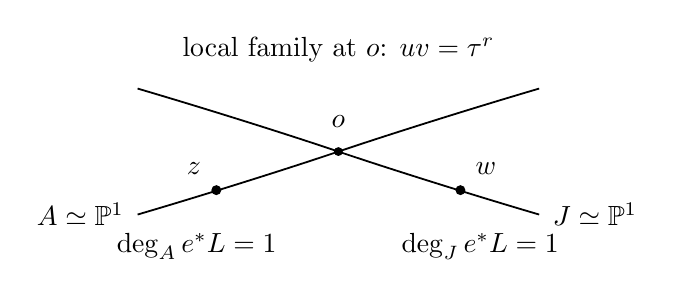
\begin{tikzpicture}[x=1cm,y=1cm,>=stealth]
  \draw[line width=0.65pt] (-2.55,-.80) .. controls (-1.7,-.55) and
    (-.65,-.22) .. (0,0) .. controls (.65,.22) and (1.7,.55) .. (2.55,.80);
  \draw[line width=0.65pt] (-2.55,.80) .. controls (-1.7,.55) and
    (-.65,.22) .. (0,0) .. controls (.65,-.22) and (1.7,-.55) .. (2.55,-.80);
  \node[anchor=east] at (-2.60,-.80) {$A\simeq\PP^1$};
  \node[anchor=west] at (2.60,-.80) {$J\simeq\PP^1$};
  \node at (-1.8,-1.20) {$\deg_A e^*L=1$};
  \node at (1.8,-1.20) {$\deg_J e^*L=1$};
  \fill (0,0) circle (1.6pt);
  \node[above=5pt] at (0,0) {$o$};
  \fill (-1.55,-.49) circle (1.8pt);
  \node[above left=2pt] at (-1.55,-.49) {$z$};
  \fill (1.55,-.49) circle (1.8pt);
  \node[above right=2pt] at (1.55,-.49) {$w$};
  \node at (0,1.30) {local family at $o$: $uv=\tau^r$};
\end{tikzpicture}
\caption{The split special source $A\cup J$, shown schematically.
The two crossing curves represent the rational components of contact
degree one. Their square has component types $A\times A$, $A\times J$,
$J\times A$ and $J\times J$.
The displayed pair $(z,w)$ lies in the mixed component $A\times J$
of the source square; this is one of the two component types where
the bivector may have a pole. The evaluation points are not stability
marks: either may also lie at the node, and they may coincide.
The picture represents the source curve, not its image in $X$.
The bounds in Equation~\eqref{ext:pole-table} and the contact vanishing
of Lemma~\ref{ext:contact-order} explain the cancellation.}
\label{fig:unmarked-boundary}
\end{figure}


\begin{lemma}[Contact vanishing at a boundary trait]
\label{ext:contact-order}
On the relatively smooth locus at the generic point of either $A$
or $J$, the bundle map
$\theta d_\pi e:T_{C/R}\to e^*L$ is divisible by $\tau^r$.
\end{lemma}

\begin{proof}
Nodal fibers are Gorenstein curves. Thus $\omega_{C/R}$ is an
invertible sheaf and its formation commutes with base change
\cite[Tag \stacksTag{0E6R}]{Stacks}. Put
\[
\mathcal N=e^*L\otimes\omega_{C/R}.
\]
On either special component the dualizing degree is $-2+1=-1$,
so $\mathcal N$ has multidegree $(0,0)$. Trivializations on $A$ and
$J$ can be rescaled to agree at their common node. Hence
$\mathcal N|_{C_k}\simeq\OO_{C_k}$, with $h^0=1$ and $H^1=0$.
On the geometric generic rational curve its degree is $2-2=0$,
so its geometric generic restriction is trivial as well.

We spell out the needed cohomology and base change over $R$.
For any line bundle $\mathcal Q$ on $C$ with
$H^1(C_k,\mathcal Q|_{C_k})=0$, multiplication by $\tau$ gives
\[
0\longrightarrow\mathcal Q\xrightarrow{\ \tau\ }
\mathcal Q\longrightarrow\mathcal Q|_{C_k}\longrightarrow0.
\]
Proper coherent cohomology is finite over the Noetherian ring $R$
\cite[Section~30.19, Tag \stacksTag{02O3}]{Stacks}. The long exact sequence
and Nakayama's Lemma therefore give $H^1(C,\mathcal Q)=0$ and
\begin{equation}\label{ext:dvr-base-change}
H^0(C,\mathcal Q)/\tau H^0(C,\mathcal Q)
\simeq H^0(C_k,\mathcal Q|_{C_k}).
\end{equation}
The finite module $H^0(C,\mathcal Q)$ is torsion-free, hence free
over $R$. Its localization is the space of sections on the generic
fiber by flat base change \cite[Section~30.5, Tag \stacksTag{02KE}]{Stacks}.
If $\mathcal Q|_{C_k}$ is globally generated, the evaluation
cokernel vanishes on the special fiber by
\eqref{ext:dvr-base-change} and Nakayama. Its support is proper
over $R$, so if nonempty it would meet the special fiber. Thus
evaluation is surjective everywhere.

Apply this to $\mathcal N$. Its pushforward is free of rank one,
and evaluation is a surjection between line bundles and hence an
isomorphism. In particular there is a nowhere-vanishing global
generator $m$ of $\mathcal N$.

The pullback of the contact form, followed by the natural
differential-to-dualizing map, is
\[
e^*L^{-1}\longrightarrow\Omega^1_{C/R}
\longrightarrow\omega_{C/R}.
\]
Equivalently it is a section $\eta$ of $\mathcal N$. There is
therefore a scalar $h_R\in R$ such that
\begin{equation}\label{ext:eta}
\eta=h_Rm.
\end{equation}
After completing the coherent map $\Omega^1_{C/R}\to\omega_{C/R}$ at
the node, a dualizing generator in $Q$ is represented by
$\gamma=du/u=-dv/v$. The canonical map sends
$du$ to $u\gamma$ and $dv$ to $-v\gamma$. This follows either
from the hypersurface dualizing formula or by checking on the two
smooth coordinate charts; the expressions respect
$v\,du+u\,dv=0$ and extend in the invertible dualizing sheaf.
In a local frame of $e^*L$, the coefficient of $\eta$ consequently
belongs to $(u,v)\subset Q$. Write $m=c$ times the product of this
frame with $\gamma$, where $c\in Q^\times$. The coefficient of
$\eta=h_Rm$ is $h_Rc$; multiplying by $c^{-1}$ preserves the ideal
$(u,v)$. Thus \eqref{ext:eta} implies
\begin{equation}\label{ext:ideal-intersection}
h_R\in (u,v)\cap R=(\tau^r).
\end{equation}
The ideal intersection is exact: $Q/(u,v)=R/(\tau^r)$.
At either component generic point, $m$ is a unit and $\tau$ has
order one. Moreover $\Omega^1_{C/R}\to\omega_{C/R}$ is an
isomorphism there, since that point is relatively smooth. Thus
\eqref{ext:ideal-intersection} gives the claimed order for the actual
contact differential on both components.
\end{proof}

\subsection{A contraction and the possible tensor poles}

To measure the possible poles of $\mathfrak b$, we identify the generic
source with $\PP^1$ by a morphism that preserves one special component
and contracts the other. The invariant tensor on $\PP^1$ is regular.
Transporting it to the source uses the inverse differential of this
morphism, whose vanishing orders will therefore bound the poles.

Choose a $k$-point of $A\setminus\{o\}$. Smoothness at that point
and henselianity give a section $\sigma:\operatorname{Spec}R\to C$
through it. Its image lies in the relatively smooth locus and is a
Cartier divisor. The line bundle $\OO_C(\sigma)$ has multidegree
$(1,0)$ on $A\cup J$. Its sections on $A$ extend uniquely as constant
sections on $J$ with matching value at $o$. This proves global
generation, $h^0=2$, and $H^1=0$ on the special fiber, for example
by the normalization sequence. The argument
\eqref{ext:dvr-base-change} gives a free rank-two pushforward and
surjective evaluation on $C$. Choosing a basis defines
\begin{equation}\label{ext:contraction}
\phi:C\longrightarrow\PP^1_R.
\end{equation}
It is an isomorphism on $A$ and contracts $J$. On the generic fiber
the line bundle has degree one, and its complete linear system is
an isomorphism to $\PP^1_{\operatorname{Frac}(R)}$: this may be
checked after an algebraic closure and then descended. Thus no
split-conic assumption on the original generic source was needed.

The differential of \eqref{ext:contraction}, composed with
$\Omega^1_{C/R}\to\omega_{C/R}$, is a section
\[
\delta_\phi\in H^0(C,\mathcal M),\qquad
\mathcal M=\omega_{C/R}\otimes\phi^*T_{\PP^1_R/R}.
\]
It is nowhere zero on the entire generic fiber, because $\phi$ is
an isomorphism there. Its zero divisor is therefore effective and
vertical. Write its Weil divisor on the normal surface $C$ as
\begin{equation}\label{ext:differential-divisor}
\operatorname{div}(\delta_\phi)=b_AA+b_JJ.
\end{equation}
At the generic point of $A$ the ordinary differential of $\phi|_A$
is nonzero, so $b_A=0$.

\begin{lemma}[The contracted-component order]
\label{ext:differential-order}
With the notation above, $b_J=r$.
\end{lemma}

\begin{proof}
Set $b=b_J$ and normalize the generic order along $J$ first:
\[
\delta'=\tau^{-b}\delta_\phi.
\]
This rational section has order zero in the component DVR of $J$.
It therefore has a well-defined nonzero \emph{generic restriction}
$s_J$ to $J$, a rational section of $\mathcal M|_J$. This operation
means reduction of a unit in that DVR, and is not the usual residue
of a meromorphic differential. At any point of $J\setminus\{o\}$,
the local Weil divisor of $\delta'$ is zero. In a local line frame,
its coefficient and inverse are regular by normality, so $s_J$ has
neither zero nor pole there. Its divisor on $J$ is supported at $o$.

We compute the order at $o$ without restricting a section having a
pole along $J$. First the completed local ring $Q$ in
\eqref{ext:node} is normal. It is a hypersurface over a regular
complete DVR, hence Cohen--Macaulay. A prime containing both $u,v$
also contains $\tau$ and is the height-two maximal ideal. Thus at a
height-one prime one of $u,v$ is invertible, and the hypersurface is
regular there, as its corresponding partial derivative is a unit.
Serre's criterion proves normality; as a local normal ring it is a
domain. In this ring,
\begin{equation}\label{ext:local-divisors}
\operatorname{div}(v)=rA,\qquad
\operatorname{div}(\tau)=A+J.
\end{equation}
For example, at the generic point of $A$, $u$ is a unit and
$v=\tau^r/u$; on $J$, $v$ is a unit. There are no horizontal
components in the divisor of $v$, since $uv=\tau^r$.

Choose a frame of $\mathcal M$ in the local ring
$\OO_{C,o}$, and let $a$ be the coefficient of $\delta_\phi$.
Since $\delta_\phi$ is nowhere zero on the entire generic fiber,
$a$ and $a^{-1}$ belong to $\OO_{C,o}[1/\tau]$. Their images are
therefore units of $Q[1/\tau]$: every height-one prime of $Q$
avoiding $\tau$ has valuation zero on $a$. In particular completion
introduces no horizontal zero or pole. The two height-one primes containing $\tau$
are the component primes $A$ and $J$. Their DVRs dominate the
corresponding component DVRs of $\OO_{C,o}$, with $\tau$ of order
one in both rings because the special fibers are reduced. A local
expression $a=\tau^j a_0$ with $a_0$ a unit therefore retains its
order $j$, since the image of $a_0$ is still a unit.
Consequently, for the coefficient $f=\tau^{-b}a$ of $\delta'$ in
the completed frame,
\[
\operatorname{div}_Q(f)=-bA.
\]
It follows from \eqref{ext:local-divisors} that $f^rv^b$ has zero
valuation at every height-one prime of $Q$. A normal Noetherian
domain is the intersection of its height-one local rings inside
its fraction field \cite[Tag \stacksTag{031T}]{Stacks}. Applying this to both
the function and its inverse gives
\begin{equation}\label{ext:unit-equation}
f^r=v^{-b}\varepsilon,\qquad \varepsilon\in Q^\times.
\end{equation}

Now reduce \eqref{ext:unit-equation} at the generic point of $J$.
This reduction is legitimate because $f$ has order zero there.
The image of $v$ is a parameter on the smooth curve $J$ at $o$,
and the image of $\varepsilon$ is a unit of $k[[v]]$. Hence
$s_J^{\otimes r}$ has order $-b$ at $o$. It has no other zero or
pole. On the other hand,
\[
\deg(\mathcal M|_J)
 =\deg(\omega_{C/R}|_J)
   +\deg(\phi^*T_{\PP^1_R/R}|_J)=-1+0=-1.
\]
The degree of the divisor of $s_J^{\otimes r}$ is therefore $-r$.
Thus $-b=-r$, proving $b_J=r$. The proof only used the Weil
divisors of the components; it did not assume that $A$ or $J$ is
Cartier when $r>1$.
\end{proof}

\subsection{The four product components and extension}

The special fiber of $C\times_R C$ has the four irreducible
components
\[
A\times A,\qquad A\times J,\qquad
J\times A,\qquad J\times J,
\]
where products in this display are over $k$. At each of their
generic points both source variables are relatively smooth. Thus
there are two ordinary relative tangent lines in which to measure
the order of $\mathfrak b$. The local ring of the product at such
a generic point is a DVR with uniformizer $\tau$. Pullback from a
component generic point of $C$ preserves order, since it sends
$\tau$ to this same uniformizer and a unit to a unit.

On the generic fiber, invariance of the canonical tensor gives
\begin{equation}\label{ext:contracted-bivector}
(d\phi\otimes d\phi)(\mathfrak b)
  =(\phi\times\phi)^*\mathfrak b_{\PP^1_R}.
\end{equation}
The right-hand side is regular. At these relatively smooth points,
the component orders of $d\phi$ are the orders of $\delta_\phi$:
they are $0$ on $A$ and $r$ on $J$, by
Lemma~\ref{ext:differential-order}. Inverting the two differentials
in \eqref{ext:contracted-bivector} therefore costs no order on
$A\times A$, and at most $r$ on either mixed component. For
$J\times J$, repeat the construction with a section through a
smooth point of $J$, obtaining a contraction that preserves $J$
and contracts $A$. Both differential orders on $J\times J$ are
then zero. Altogether the bounds are
\begin{equation}\label{ext:pole-table}
\begin{array}{c|cccc}
\text{component}&A\times A&A\times J&J\times A&J\times J\\ \hline
\operatorname{ord}(\mathfrak b)\text{ at least}
 &0&-r&-r&0.
\end{array}
\end{equation}
Each same-component product uses a contraction preserving that
component. On each mixed product, exactly one inverse differential
contributes a possible pole of order $r$.

Lemma~\ref{ext:contact-order} supplies order at least $r$ for the
contact differential in \emph{either} variable. For $W_{12}^\circ$
use the contact differential in the second variable, and for
$W_{21}^\circ$ use it in the first. In each case this cancels the
only possible negative order in \eqref{ext:pole-table}. The remaining
ordinary differential $d_\pi e$ is a regular homomorphism at these
relatively smooth generic points. Thus each vector section has
nonnegative order on all four product components.

We have checked every height-one point not already in
$\mathcal D^\circ$. On a normal Noetherian scheme, a rational
section of a locally free sheaf which is regular at all height-one
points is regular everywhere: trivialize the sheaf and use the
normal-domain intersection criterion. Apply this on the scheme
charts of $\mathcal D$ to the locally free bundles
$\widetilde p^*\mathcal E_{12}$ and
$\widetilde p^*\mathcal E_{21}$. It yields unique sections
\begin{equation}\label{ext:extended-vectors}
\widetilde W_{12}\in
H^0(\mathcal D,\widetilde p^*\mathcal E_{12}),\qquad
\widetilde W_{21}\in
H^0(\mathcal D,\widetilde p^*\mathcal E_{21}).
\end{equation}
Uniqueness makes the extensions agree on overlaps and respect the
stack descent data. This step uses local freeness of the
\emph{target} bundles; it asserts no local freeness of a relative
tangent sheaf at a node. Nodes, coincident points, and all strata
of higher codimension are included by this normal extension.

The two contact values of \eqref{ext:extended-vectors} agree on
the dense smooth-source open and therefore everywhere. Denote
their common value by $\widetilde\xi$. The involution of
$\mathcal D$ interchanging its two factors likewise preserves
$\widetilde\xi$, with the canonical interchange of the two line
factors, because it does so on that dense open.

\subsection{Coarse space and the full family identity}

Let $\rho:\mathcal D\to Y$ be the coarse moduli morphism. We use
the following precise form of the coarse-space Theorem: an
algebraic stack locally of finite presentation over a scheme,
with quasi-compact separated diagonal and finite inertia, has a coarse
algebraic space; its coarse
morphism is proper, surjective and quasi-finite, the coarse space
is separated when the stack is separated, and is locally of finite
type over a locally Noetherian base. Moreover
\begin{equation}\label{ext:coarse-functions}
\rho_*\OO_{\mathcal D}=\OO_Y
\end{equation}
on the \'etale site
\cite[Theorem~1.1 and the following note]{ConradKM}.
Here $\mathcal D$ is a proper finite-type Deligne--Mumford stack,
so its diagonal is quasi-compact and separated, its inertia is finite,
and the stated hypotheses hold. It follows
that $Y$ is of finite type and separated over $\CC$; universal
closedness follows from properness of $\mathcal D$ and surjectivity
of its coarse morphism, also after every base change. Thus $Y$ is
proper. Its underlying space is irreducible as the image of the
integral stack $\mathcal D$, and \eqref{ext:coarse-functions} makes
it reduced. It is therefore an integral algebraic space.

By the universal property, $\widetilde p$ factors uniquely as
$p\rho$ for a morphism $p:Y\to X\times X$, which is dominant.
The involution of $\mathcal D$ similarly descends to an involution
$\iota$ of $Y$. Both bundles in \eqref{ext:extended-vectors} are
pullbacks of bundles from $Y$, namely $p^*\mathcal E_{12}$ and
$p^*\mathcal E_{21}$. The projection formula and
\eqref{ext:coarse-functions} give, for either bundle $\mathcal V$,
\[
H^0(\mathcal D,\rho^*\mathcal V)=H^0(Y,\mathcal V).
\]
This identity can equally be checked on \'etale opens trivializing
$\mathcal V$, where it is \eqref{ext:coarse-functions} in each
coordinate. Thus \eqref{ext:extended-vectors} descend to the desired
$W_{12},W_{21}$, with the same equality of contact values and the
same symmetry. No descent assertion about arbitrary bundles on a
stack is being used.

Finally take $j=\rho\widetilde j$ in
\eqref{ext:hom-to-stack}. Its entire source lies over smooth source
curves, so the original definition \eqref{ext:initial-vectors}
gives \eqref{ext:hom-vectors} and \eqref{ext:hom-identity} on the
full neighborhood $\mathcal H$. This completes the proof of
Proposition~\ref{ext:moving-pair}.

\section{Descent of the common contact value}
\label{des:section}

The common contact value constructed in Section~\ref{ext:section}
is a section on a proper family over $X\times X$. We must show that its
value depends only on the two points of $X$. Properness first gives
finitely many possible values over each pair. The two vector lifts
then control these values along contact lines in opposite factors.
These tests exclude branching; purity and simple connectedness then
give a single value. We formulate this descent independently of the
stable-map construction. Throughout this section put
\[
Z=X\times X,\qquad M=L\boxtimes L.
\]

\begin{proposition}[Contact-value descent on the square]
\label{des:descent}
Let $X$ be a smooth simply connected complex projective contact Fano
manifold with $\Pic(X)=\ZZ[L]$. Assume that a family of free contact
lines covers a dense open subset of $X$. Let $p:Y\to Z$ be dominant,
where $Y$ is a proper integral algebraic space over $\CC$. Suppose that
there are regular sections
\[
W_{12}\in H^0\bigl(Y,p^*(T_X\boxtimes L)\bigr),\qquad
W_{21}\in H^0\bigl(Y,p^*(L\boxtimes T_X)\bigr)
\]
with the same contact value
\begin{equation}\label{des:common-value}
\xi=(\theta\boxtimes 1)(W_{12})
    =(1\boxtimes\theta)(W_{21})\in H^0(Y,p^*M).
\end{equation}
Then there is a unique section $B\in H^0(Z,M)$ such that $p^*B=\xi$.
\end{proposition}

\begin{proof}
\noindent\textbf{The finite image and its normalization.}
The section $\xi$ defines a morphism
$a:Y\to\Tot(M)$ over $Z$. It is proper: its graph is closed because
$\Tot(M)$ is separated over $\CC$, and projection from
$Y\times\Tot(M)$ is proper. Let $S_0$ be its reduced closed image.
This is an integral scheme, and $a$ factors through a proper surjection
$Y\to S_0$, since $Y$ is reduced.

The scheme $S_0$ is proper over $\CC$. Indeed it is separated and of
finite type, and universal closedness descends along the surjection
$Y\to S_0$: after any base change, a closed subset of $S_0$ has
closed inverse image in $Y$ with the same image in the base. Since
$S_0$ is closed in the line-bundle total space, $q_0:S_0\to Z$ is
affine. It is also proper, hence finite. Dominance of $p$ makes $q_0$
surjective.

Let $\nu:S\to S_0$ be the normalization and put $q=q_0\nu$.
A scheme of finite type over $\CC$ is Nagata, so normalization is
finite \cite[Tags \stacksTag{035B} and \stacksTag{035S}]{Stacks}. Thus $q$ is a finite
dominant morphism of integral schemes, $S$ is normal, and $q$ is
generically \'etale by characteristic zero.
We require an open set in the \emph{base} on which normalization
causes no change. The morphism $\nu$ is an isomorphism over a dense
open $V\subset S_0$. The finite image $q_0(S_0\setminus V)$ is a
proper closed subset of $Z$, since finite maps preserve the dimension
of closed subsets. The image under $q$ of its non-\'etale locus is
likewise proper and closed. Deleting both images gives a dense open
\begin{equation}\label{des:base-open}
U\subset Z\quad\text{such that}\quad
S\times_ZU\simeq S_0\times_ZU\longrightarrow U
\text{ is finite \'etale}.
\end{equation}
No morphism from $Y$ to the normalization $S$ is required.

\medskip
\noindent\textbf{Every generic sheet splits over either type of line.}
Choose a smooth irreducible open family $H$ of parametrized free contact
lines with smooth dominant evaluation
\[
\operatorname{ev}:H\times\PP^1\longrightarrow X.
\]
This is possible by Corollary~\ref{lines:free-cover}: freeness gives
$H^1(\PP^1,f^*T_X(-t))=0$ for every $t$, so evaluation is smooth at
every pair $(f,t)$ on the chosen open of the Hom scheme. For each
$f\in H$, let $P_f$ be the positive part of $f^*T_X$. Thus
\begin{equation}\label{des:line-quotient}
f^*T_X/P_f\simeq\OO_{\PP^1}^{\oplus r_f},
\qquad \theta(P_f)=0.
\end{equation}
The second assertion is Lemma~\ref{lines:positive}.


Consider a map
\[
c:\PP^1\longrightarrow Z,\qquad c=(f,y),\quad f\in H,
\]
whose image meets $U$. Set $T=\PP^1\times_ZY$, and let
$D\subset T$ be any reduced irreducible component dominating
$\PP^1$, with projection $\pi_D:D\to\PP^1$. It is a proper
integral algebraic space over $\CC$, and
$H^0(D,\OO_D)=\CC$. For the latter assertion, a regular function
gives a morphism to $\PP^1$ whose proper irreducible image avoids
infinity, hence is a point.

Pull $W_{12}$ back to $D$ and project to
\[
\pi_D^*\bigl((f^*T_X/P_f)\otimes L_y\bigr).
\]
In a global trivialization this section is a constant vector, by
\eqref{des:line-quotient} and the preceding assertion about functions.
The contact map factors through this quotient. Consequently there
exists a section
\begin{equation}\label{des:component-section}
a_D\in H^0(\PP^1,c^*M),\qquad
\xi|_D=\pi_D^*a_D.
\end{equation}
For the other type $c=(y,f)$, the identical argument uses $W_{21}$
and proves the same assertion.

We spell out why this accounts for \emph{all} sheets. Write
$K=\CC(\PP^1)$ and $\eta=\Spec K$. The surjection $Y\to S_0$
remains surjective after base change, so
\[
T_\eta\longrightarrow (\PP^1\times_ZS_0)_\eta
\]
is surjective. There are finitely many irreducible components of $T$;
the components that do not dominate $\PP^1$ disappear over $\eta$.
Every point of $T_\eta$ therefore belongs to the generic fiber of one
of the components $D$ just considered. Trivialize $c^*M$ over $K$.
Then $(\PP^1\times_ZS_0)_\eta$ is a finite closed subscheme of
$\mathbb A^1_K$, and \eqref{des:component-section} puts the image of
$D_\eta$ at the $K$-rational point whose coordinate is $a_D(\eta)$.
Indeed the induced map from the coordinate algebra $K[\zeta]$ sends
$\zeta$ to the scalar $a_D(\eta)\in K$, so it factors through
$K[\zeta]/(\zeta-a_D(\eta))=K$. This does not require a
$K$-rational point of $D_\eta$.
Surjectivity shows that every point of this finite subscheme is
$K$-rational. By \eqref{des:base-open} the subscheme agrees with
$(\PP^1\times_ZS)_\eta$ and is finite \'etale, hence reduced.
Its algebra is therefore a product of copies of $K$.

In particular, for \emph{every} $c$ of either type that meets $U$,
\begin{equation}\label{des:all-sheets}
\begin{gathered}
C\subset(\PP^1\times_ZS)_{\mathrm{red}}\text{ an irreducible component},
\quad C\longrightarrow\PP^1\text{ dominant}\\
\Longrightarrow\qquad \deg(C^\nu/\PP^1)=1,
\end{gathered}
\end{equation}
where $C^\nu$ denotes the normalization of $C$.
This conclusion uses neither flatness of $T$ nor connectedness or
reducedness of its fibers. The embedding of $S_0$ in a line bundle is
what converts the componentwise contact values into rational sheets.

\medskip
\noindent\textbf{The local model at a ramification divisor.}
Suppose that $q$ is not unramified at the generic point of some
prime divisor $R\subset S$. Its image is a prime divisor
$\Delta\subset Z$, since $q$ is finite. Put $N=\dim Z=2\dim X$.
There is a dense smooth open $\Delta^0\subset\Delta$ such that every
point above $\Delta^0$ is smooth in $S$, and the reduced divisors
$R_i$ above $\Delta$ are smooth, disjoint, and \'etale over
$\Delta^0$. To obtain this open, delete from $\Delta$ the finite image
of $\operatorname{Sing}(S)\cap q^{-1}(\Delta)$ and those of the
singular loci of the $R_i$, their pairwise intersections, and the
non-\'etale loci of $R_i\to\Delta$, as well as the singular locus
of $\Delta$. These are proper closed subsets
of $\Delta$: normality makes $S$ regular at every divisorial generic
point, and the finite maps of reduced divisors are generically
separable in characteristic zero.

At a point $s\in R_i$ over $x\in\Delta^0$, choose local analytic
coordinates $(x_1,\ldots,x_N)$ on $Z$ with $\Delta=(x_1=0)$.
If $z_1$ locally defines $R_i$, then
$q^*x_1=u z_1^{e_i}$ for a unit $u$. Absorb an analytic $e_i$-th
root of $u$ into $z_1$ and take $q^*x_2,\ldots,q^*x_N$ as the
remaining coordinates; their restrictions are coordinates along
$R_i$ because its map to $\Delta^0$ is \'etale. The map becomes
\begin{equation}\label{des:branch-model}
(z_1,\ldots,z_N)\longmapsto
(z_1^{e_i},z_2,\ldots,z_N).
\end{equation}
At least one $e_i$ is greater than one. Otherwise this model would
make $q$ unramified at every generic point over $\Delta$, contrary
to the choice of $R$. Each point of $\Delta^0$ has a preimage on
such a ramified $R_i$, since $R_i\to\Delta$ is finite surjective.

\medskip
\noindent\textbf{A test line detects every possible divisor.}
Let $d=\dim X$. If $\Delta\to X$ under the second projection is
dominant, then for general $y\in X$ its intersection with
$X\times\{y\}$ is a nonempty effective Cartier divisor
$\Delta_y$ on $X$. It is Cartier by restricting a local equation of
$\Delta$ to a fiber not contained in $\Delta$, and its nonemptiness
and dimension $d-1$ follow from properness and the fiber dimension
Theorem. Write $\OO_X(\Delta_y)=L^{\otimes a}$. A nonzero effective
divisor has positive intersection with $L^{d-1}$, so $a>0$.
For every contact line $f$ not contained in $\Delta_y$,
\[
\deg f^*\OO_X(\Delta_y)=a\deg f^*L=a>0.
\]
Thus a general test line of the first type $(f,y)$ meets $\Delta$.

If $\Delta$ does not dominate the second factor, its closed image
$D\subset X$ has dimension at least $d-1$, because
$\dim\Delta=2d-1$ and its fibers have dimension at most $d$.
Hence $D$ is a prime divisor, and the inclusion
$\Delta\subset X\times D$ between irreducible varieties of the
same dimension is equality. In this case $\OO_X(D)=L^{\otimes a}$
with $a>0$ by the same intersection argument, and a general line of
the second type $(y,f)$ meets $\Delta=X\times D$.

For completeness, the required general-position assertions concern
the whole chosen line family, whose evaluation need only be dominant.
For either type let $P=H\times X$, put $m=\dim P$, and denote the
universal evaluation by
\[
E:P\times\PP^1\longrightarrow Z.
\]
It is smooth and dominant. If $A=\Delta\setminus\Delta^0$, then
$A$ is closed of codimension at least two in $Z$ and
\[
\dim E^{-1}(A)\leq m-1.
\]
Projection to $P$ is proper, so the image of $E^{-1}(A)$ is a
proper closed subset of $P$. A general test line therefore avoids
$A$. The scheme $E^{-1}(\Delta^0)$ is smooth of pure dimension $m$.
Discard the closures of the images of its nondominating components,
and apply generic
smoothness to the projections of its dominating components to $P$.
For general parameters their fibers are smooth of dimension zero.
These fibers are the inverse images of $\Delta^0$ on the test line,
so all intersections are transverse. Finally, meeting $U$ and not
being contained in $\Delta$ are nonempty open conditions on $P$:
they are images under the open projection $P\times\PP^1\to P$ of
the corresponding nonempty open inverse images under $E$.
All these open conditions hold simultaneously because $P$ is
irreducible. For the type selected in the preceding two paragraphs,
positive intersection ensures at least one intersection with
$\Delta^0$.

\medskip
\noindent\textbf{Ramification contradicts the split sheets.}
Choose this test line $c$, a transverse intersection $c(t_0)\in
\Delta^0$, and a ramified point $s$ above it. In
\eqref{des:branch-model} let $e=e_i>1$ and take a local parameter
$t$ at $t_0$. Eliminating the tangential coordinates, the analytic
local ring of $\PP^1\times_ZS$ at $(t_0,s)$ is
\begin{equation}\label{des:pullback-germ}
\CC\{z_1,t\}/(z_1^e-a(t)),\qquad
a(0)=0,\quad a'(0)\ne0.
\end{equation}
It is isomorphic to $\CC\{z_1\}$ by the analytic inverse function
Theorem. Thus this pullback germ itself is smooth, reduced, and
irreducible, and $t$ has order $e$ on it. In particular no vertical
or embedded component passes through this germ, whatever happens
elsewhere in the finite pullback. The unique reduced irreducible
component through it dominates $\PP^1$. Its normalization is
unchanged near this smooth point, and the resulting finite map of
normal curves has ramification index $e$. The degree of that map is
at least $e$, by the degree formula for a fiber of a finite map of
smooth curves. This contradicts \eqref{des:all-sheets}. We have proved
that $q$ is unramified at every codimension-one point of $S$.

\medskip
\noindent\textbf{Purity and simple connectedness.}
We check the local hypotheses of purity at an arbitrary nongeneric
point $s\in S$, with $z=q(s)$. Both schemes are Noetherian,
$\OO_{S,s}$ is normal, $\OO_{Z,z}$ is regular, and $q$ is
quasi-finite at $s$ because it is finite. Moreover
\[
\dim\OO_{S,s}=\dim\OO_{Z,z}>0.
\]
Indeed, on affine charts the corresponding finite extension of
domains has going down because the base domain is integrally closed
\cite[Proposition 10.38.7, Tag \stacksTag{00H8}]{Stacks}.
Going down and incomparability of primes in an integral extension
give equality of the heights of corresponding primes, including
nonclosed points. For every generization $s'$ of $s$ with
$\dim\OO_{S,s'}=1$, the map $q$ is unramified at $s'$ by the
preceding paragraph. These are precisely the local hypotheses of
purity of the branch locus, which makes $q$ \'etale at $s$
\cite[Lemma 58.21.4, Tag \stacksTag{0BMB}]{Stacks}. The generic point
is already \'etale by separability. In particular flatness is a
conclusion here, not a premise about $q$ or its line pullbacks.

The analytic space $Z^{\mathrm{an}}=X^{\mathrm{an}}\times
X^{\mathrm{an}}$ is simply connected. The finite \'etale map $q$
analytifies to a finite covering, which is connected because $S$ is
integral. It has degree one. Consequently $S_0\to Z$ is finite
birational and hence an isomorphism, since $Z$ is normal
\cite[Lemma 29.55.8, Tag \stacksTag{0AB1}]{Stacks}. Its closed inclusion into
$\Tot(M)$ is the graph of a global section $B$ with $p^*B=\xi$.
Finally, pullback of sections of a line bundle along a dominant map
of integral spaces is injective. This proves uniqueness.
\end{proof}

\begin{corollary}[Symmetry and the full local family]
\label{des:family}
Apply Proposition~\ref{des:descent} to the space and tensors of
Proposition~\ref{ext:moving-pair}. The resulting section
$B\in H^0(X\times X,L\boxtimes L)$ is symmetric under exchange of
the factors, using the canonical exchange of the two line factors.
For the full neighborhood $\mathcal H$ of $g$ in the space of
parametrized degree-two maps provided there, one has
\begin{equation}\label{des:family-identity}
B\bigl(h(z),h(w)\bigr)
=(z-w)^2\,\theta\bigl(dh(\partial_z)\bigr)
       \otimes\theta\bigl(dh(\partial_w)\bigr),
\qquad h\in\mathcal H.
\end{equation}
This identity holds for all pairs of source points, including the
diagonal; its displayed expression uses any common affine coordinate.
\end{corollary}

\begin{proof}
Let $\sigma:Z\to Z$ exchange the two factors, and let
$\iota:Y\to Y$ be the involution in
Proposition~\ref{ext:moving-pair}. Under the canonical line-bundle
identifications, $p\iota=\sigma p$ and $\iota^*\xi=\xi$. Hence
\[
p^*(\sigma^*B)=\iota^*(p^*B)=\iota^*\xi=\xi=p^*B.
\]
Dominance of $p$ gives $\sigma^*B=B$.

The equality $p^*B=\xi$ pulls back along the morphism
$\mathcal H\times\PP^1\times\PP^1\to Y$ supplied by
Proposition~\ref{ext:moving-pair}. Its smooth-source formula
\eqref{ext:hom-identity} gives \eqref{des:family-identity}.
Here $\mathcal H$ is a neighborhood in the full Hom space by
Lemma~\ref{sm:full-germ}, so no deformation directions at $g$ are lost.
Coordinate independence
and regularity at infinity follow from the invariant tensor
$(z-w)^2\partial_z\otimes\partial_w$; its double zero on the
diagonal also proves the asserted diagonal identity.
\end{proof}

\section{Diagonal jets and contact transitivity}
\label{jet:section}

Corollary~\ref{des:family} provides a symmetric section
\[
B\in H^0(X\times X,L\boxtimes L)
\]
and the identity
\begin{equation}\label{jet:family}
B(h(z),h(w))
=(z-w)^2\theta(h'(z))\otimes\theta(h'(w))
\end{equation}
on the full neighborhood $\mathcal H$ of the very free parametrized map $g$ of
Proposition~\ref{sm:very-free}. Here $z,w$ belong to one affine
coordinate chart of $\PP^1$, and $h'$ denotes differentiation in that
coordinate. We first determine the diagonal symbol of $B$ at every
point of $X$. We then prove a criterion that applies to any compact
complex contact manifold with such a symmetric section.

\subsection{From the full family to the diagonal}

\begin{lemma}\label{jet:value-velocity}
Fix the parameter $0\in\PP^1$ and its affine coordinate. There is a
Zariski-open neighborhood $\mathcal U\subset\mathcal H$ of $g$ on which
the value--velocity morphism
\[
\mathcal U\longrightarrow T_X,
\qquad h\longmapsto\bigl(h(0),h'(0)\bigr),
\]
is smooth. Its image is open in $T_X$. Its projection is a nonempty
open subset $U\subset X$, and for each $x\in U$ the velocities of maps
in $\mathcal U$ with $h(0)=x$ form a nonempty open subset of $T_xX$.
\end{lemma}

\begin{proof}
Put $E=g^*T_X$. Every splitting summand of $E$ has degree at least
one, so $H^1(E(-2\cdot0))=0$. The exact sequence
\[
0\longrightarrow E(-2\cdot0)\longrightarrow E
\longrightarrow E|_{2\cdot0}\longrightarrow0
\]
therefore makes $H^0(E)\to H^0(E|_{2\cdot0})$ surjective.
The Hom space is smooth at $g$ and has tangent space $H^0(E)$.
In target coordinates its joint value and velocity differential is
\[
\psi\longmapsto\bigl(\psi(0),\psi'(0)\bigr),
\]
which is precisely this restriction map, expressed in the
coordinate trivialization along $g$. It is surjective. The source and
target are smooth at the points in question, so the smooth locus of this
morphism contains a Zariski-open neighborhood $\mathcal U\subset\mathcal H$
of $g$. Its image in $T_X$ is open.
Projection to $X$ and intersection with its fibers give the final
assertions.
\end{proof}

Let $\Delta\subset X\times X$ be the diagonal, let $\mathcal I$
be its ideal sheaf, and put $M=L\boxtimes L$. We identify
$\mathcal I/\mathcal I^2$ with $\Omega_X^1$ by sending the class of
$f(y)-f(x)$ to $df$. Since $\Delta$ is a regular embedding,
\begin{equation}\label{jet:symbol-bundles}
(\mathcal I^k/\mathcal I^{k+1})\otimes M|_\Delta
\simeq\Sym^k\Omega_X^1\otimes L^{\otimes2}.
\end{equation}
We write $\theta^2$ for the symmetric square of the $L$-valued
one-form $\theta$, with quadratic value $v\mapsto\theta(v)^2$.

\begin{proposition}\label{jet:diagonal}
The section $B$ vanishes to order at least two along $\Delta$, and
its second diagonal symbol is
\begin{equation}\label{jet:second-symbol}
B\in H^0(X\times X,\mathcal I^2\otimes M),
\qquad [B]_2=\theta^2
\quad\text{in }H^0(X,\Sym^2\Omega_X^1\otimes L^{\otimes2}).
\end{equation}
\end{proposition}

\begin{proof}
Choose local coordinates and one local frame $e$ of $L$, used in
both factors. Write $\theta=e\alpha$ and
$B(x,y)=b(x,y)e(x)\otimes e(y)$. Fix $x\in U$ as in
Lemma~\ref{jet:value-velocity}. Setting $z=0$ in
Equation~\eqref{jet:family}, for a nearby map with
$h(0)=x$ and $h'(0)=a$, gives
\begin{equation}\label{jet:curve-expansion}
b(x,h(w))
=w^2\alpha_x(a)\alpha_{h(w)}(h'(w))
=w^2\alpha_x(a)^2+O(w^3).
\end{equation}
The constant term proves $B|_\Delta=0$ on $U$. As this restriction
is a global holomorphic section of $L^{\otimes2}$ on connected
$X$, it vanishes everywhere.

The first symbol is now intrinsically a section of
$\Omega_X^1\otimes L^{\otimes2}$. On $U$, its value on $a$ is
the coefficient of $w$ in Equation~\eqref{jet:curve-expansion}.
That coefficient vanishes for a nonempty open set of velocities,
so the linear form is zero. The first symbol consequently
vanishes on all of $X$, again by the identity Theorem. Thus
$B$ belongs to $\mathcal I^2\otimes M$ globally.

Its second symbol is now the global section in
Equation~\eqref{jet:symbol-bundles} for $k=2$. Because the linear
term has vanished, the acceleration $h''(0)$ contributes nothing
to the coefficient of $w^2$ in Equation~\eqref{jet:curve-expansion}.
The quadratic symbol takes the value $\alpha_x(a)^2$ on a nonempty
open set of $a$, and hence equals $\alpha_x^2$ as a quadratic form.
The difference $[B]_2-\theta^2$ is a holomorphic section of the
displayed symbol bundle, zero on $U$; it is therefore zero on $X$.
Each continuation has been performed after the preceding lower
symbol vanished, so all three identities are intrinsic.
\end{proof}

\subsection{A symmetric-jet criterion}

The remainder of the argument uses only symmetry and
Equation~\eqref{jet:second-symbol}. The quadratic symbol records contact
values of tangent vectors. Symmetry determines the next Taylor term.
Differentiating this expansion in the first slot reveals the Levi form,
which will detect directions inside the contact plane. We first make this local
calculation, then use it to prove Theorem~\ref{jet:criterion}.

\begin{lemma}\label{jet:local-calculation}
Let $B$ be symmetric and satisfy Equation~\eqref{jet:second-symbol}
on a complex contact manifold. In local coordinates and a frame
as above, put $s=y-x$ and
$A_x(u,v)=(\partial_u\alpha)_x(v)$, where $\partial$ differentiates
the coefficients of $\alpha$. Then
\begin{equation}\label{jet:cubic}
b(x,x+s)=\alpha_x(s)^2+\alpha_x(s)A_x(s,s)+O(s^4).
\end{equation}
Differentiation in the first slot, with the second slot held
fixed, gives
\begin{equation}\label{jet:fixed-second}
\begin{split}
D^{(1)}_v b(x,x+s)
={}&-2\alpha_x(s)\alpha_x(v)
   +\alpha_x(s)d\alpha_x(v,s)\\
 &\hspace{8mm}-\alpha_x(v)A_x(s,s)+O(s^3).
\end{split}
\end{equation}
\end{lemma}

\begin{proof}
Write the expansion initially as
$b(x,x+s)=Q_x(s)+C_x(s)+O(s^4)$, where
$Q_x(s)=\alpha_x(s)^2$ and $C_x$ is homogeneous of degree three.
Symmetry, with the same frame in both slots, gives
\[
Q_x(s)+C_x(s)
=Q_{x+s}(-s)+C_{x+s}(-s)+O(s^4).
\]
The two terms on the right are respectively
\[
\alpha_x(s)^2+2\alpha_x(s)A_x(s,s)+O(s^4),
\qquad -C_x(s)+O(s^4).
\]
Thus $C_x(s)=\alpha_x(s)A_x(s,s)$, proving
Equation~\eqref{jet:cubic}.

For the first-slot derivative, $y$ is fixed and hence $s=y-x$
has derivative $-v$. The quadratic term contributes
\[
-2\alpha_x(s)\alpha_x(v)+2\alpha_x(s)A_x(v,s).
\]
Through degree two, the cubic term contributes only through its
arguments $s$, giving
\[
-\alpha_x(v)A_x(s,s)
-\alpha_x(s)\bigl(A_x(v,s)+A_x(s,v)\bigr).
\]
Their sum is Equation~\eqref{jet:fixed-second}, since
$d\alpha_x(v,s)=A_x(v,s)-A_x(s,v)$. Differentiating the holomorphic
remainder with $y$ fixed lowers its order by at most one.

These scalar formulas also keep track of changes of line frame.
If $e'=q e$ and $\rho=q^{-1}$, then
\[
\alpha'=\rho\alpha,
\qquad b'(x,y)=\rho(x)\rho(y)b(x,y).
\]
The cubic coefficient transforms as
\[
C'_x(s)=\rho(x)^2 C_x(s)
+\rho(x)d\rho_x(s)\alpha_x(s)^2
=\alpha'_x(s)(\partial_s\alpha')_x(s).
\]
Moreover the derivative at fixed $y$ transforms by
\[
D^{(1)}_v b'
=\rho(x)\rho(y)D^{(1)}_v b
+d\rho_x(v)\rho(y)b.
\]
In particular, it includes exactly the first-slot frame term.
The cubic is a coordinate expression; the symbol in
Equation~\eqref{jet:second-symbol} is intrinsic.
\end{proof}

\begin{lemma}[Contact Hamiltonians]\label{jet:hamiltonian}
On a complex contact manifold, contact value identifies the
holomorphic vector fields preserving $F$ with $H^0(X,L)$
\cite[Proposition~2.1]{LeBrun1995}.
For $a\in H^0(X,L)$, write $K_a$ for the corresponding field.
In a frame $\theta=e\alpha$, $a=e f$, it is characterized by
\begin{equation}\label{jet:hamiltonian-equations}
\alpha(K_a)=f,
\qquad df(w)+d\alpha(K_a,w)=0\quad(w\in F).
\end{equation}
Its value at a point depends only on the ordinary first jet of $a$.
\end{lemma}

\begin{proof}
Choose a local holomorphic field $R$ with $\alpha(R)=1$ and
write $K_a=fR+Z$ with $Z\in F$. The second equation determines
$Z$ uniquely and holomorphically because $d\alpha|_F$ is
nondegenerate. Cartan's formula identifies that equation with
$(\mathcal L_{K_a}\alpha)|_F=0$, equivalently
$[K_a,F]\subset F$. It also proves that every field preserving
$F$ satisfies the equations for its contact value.

For completeness, under a frame change
$\alpha'=\rho\alpha$, $f'=\rho f$, and for $w\in F$, we have
\[
df'(w)+d\alpha'(K_a,w)
=\rho\bigl(df(w)+d\alpha(K_a,w)\bigr),
\]
since the extra terms are
$d\rho(w)f-d\rho(w)\alpha(K_a)=0$. The first equation transforms
by the same factor. Uniqueness therefore makes the local fields
independent of the chosen frame and lift $R$, and they glue.
The displayed equations use only $f(x)$ and $df_x$ to determine
$K_a(x)$. This also proves naturality under contact automorphisms.
\end{proof}

\begin{theorem}[Symmetric-jet criterion]\label{jet:criterion}
Let $X$ be a connected compact complex contact manifold with
contact quotient $\theta:T_X\to L$, and let $\mathcal I_\Delta$
be the ideal sheaf of the diagonal in $X\times X$.
Suppose that a symmetric section $B\in H^0(X\times X,L\boxtimes L)$
satisfies
\[
\begin{gathered}
B\in H^0(X\times X,\mathcal I_\Delta^2\otimes(L\boxtimes L)),\\
[B]_2=\theta^2
\quad\text{in }H^0(X,\Sym^2\Omega_X^1\otimes L^{\otimes2}).
\end{gathered}
\]
Then the ordinary first-jet evaluation map
\begin{equation}\label{jet:jet-generation}
H^0(X,L)\longrightarrow J_x^1L
\end{equation}
is surjective at every $x\in X$. Global contact vector fields
span $T_xX$ at every point, and the identity component of the
holomorphic contact automorphism group acts transitively.
\end{theorem}

\begin{proof}
Put $d=\dim X$ and $V=H^0(X,L)$, a finite-dimensional vector space
by compactness. Write $B_x$ for the restriction of $B$ to
$\{x\}\times X$, viewed as an element of $L_x\otimes V$.
Point evaluations followed by fiber functionals span $V^*$, since
only the zero section vanishes at every point. Choose a basis
$\varepsilon_1,\ldots,\varepsilon_r$ among these functionals, and let
$s_1,\ldots,s_r$ be its dual basis in $V$. Contracting the second
factor of $B$ by $\varepsilon_j$ gives a global section $t_j$ of $L$
on the first factor. For each $x$, all the $\varepsilon_j$ kill
$B_x-\sum_jt_j(x)\otimes s_j$, so that difference is zero. Hence
$B=\sum_jt_j\otimes s_j$, and in particular
\[
B\in H^0(X,L)\otimes V
=H^0(X,L\otimes(V\otimes\OO_X)).
\]
For each $x$, the vector $B_x\in L_x\otimes V$ is nonzero.
Indeed $B_x=0$ would say that $B(x,y)$ vanishes identically in $y$,
contradicting its nonzero quadratic term $\alpha_x(s)^2$.
Thus $B$ gives a line subbundle and a holomorphic map
\begin{equation}\label{jet:beta}
L^{-1}\hookrightarrow V\otimes\OO_X,
\qquad \beta:X\longrightarrow\PP(V),
\qquad \beta^*\OO_{\PP(V)}(1)\simeq L.
\end{equation}

We claim that $\beta$ is an immersion. In a local frame write
$B=e\otimes w$, with $w$ a holomorphic $V$-valued function.
If $d\beta_x(v)=0$, then $\partial_vw(x)=k w(x)$ for a scalar
$k$, independent of the second variable. Evaluating these global
sections in the frame at $y$ gives
\begin{equation}\label{jet:kernel}
D^{(1)}_v b(x,y)=k b(x,y).
\end{equation}
The linear terms of Equation~\eqref{jet:fixed-second} imply
$\alpha_x(v)=0$, because $\alpha_x$ is a nonzero linear form.
The quadratic terms then give the polynomial identity
\[
\alpha_x(s)d\alpha_x(v,s)=k\alpha_x(s)^2.
\]
Cancelling the nonzero linear polynomial $\alpha_x(s)$ shows
$d\alpha_x(v,\cdot)=k\alpha_x$. Its restriction to $F_x$ is
zero. Since $v\in F_x$, contact nondegeneracy gives $v=0$.

We now pass explicitly from this immersion to actual global
sections. Every $\lambda\in V^*$ gives
\[
t_\lambda=(\id\otimes\lambda)B\in H^0(X,L),
\qquad (t_\lambda)_{\mathrm{loc}}=\lambda(w).
\]
If $v_1,\ldots,v_d$ is a basis of $T_xX$, the $d+1$ vectors
\[
w(x),\ \partial_{v_1}w(x),\ldots,\partial_{v_d}w(x)
\]
are linearly independent: a dependence with nonzero tangent part
would contradict immersion, and a dependence with zero tangent
part contradicts $w(x)\ne0$. Dualizing gives surjectivity of
\[
V^*\longrightarrow L_x\oplus(T_x^*X\otimes L_x),
\qquad
\lambda\longmapsto\bigl(t_\lambda(x),d(t_\lambda)_{\mathrm{loc},x}\bigr),
\]
where the target is the local-frame description of $J_x^1L$.
Recall its intrinsic exact sequence
$0\to\Omega_X^1\otimes L\to J^1L\to L\to0$.
Since every $t_\lambda$ belongs to $H^0(X,L)$, this proves
Equation~\eqref{jet:jet-generation}. No nondegeneracy of $B$ as
a tensor in $V\otimes V$ is required.

Given $u\in T_xX$, prescribe a first jet $j_x^1a$ whose scalar
representative satisfies
\[
f(x)=\alpha_x(u),
\qquad df_x|_{F_x}=-d\alpha_x(u,\cdot)|_{F_x}.
\]
Extend the prescribed covector arbitrarily from $F_x$ to $T_xX$.
First-jet surjectivity realizes this jet by a global section $a$.
Lemma~\ref{jet:hamiltonian} and uniqueness in
Equation~\eqref{jet:hamiltonian-equations} imply $K_a(x)=u$.
Thus global contact fields span every tangent space.

A global holomorphic vector field on a compact complex manifold
has a global flow for sufficiently small complex time. Compactness
allows a common time disk for all initial points, and the
inverse is supplied by negative time. For a contact field these
automorphisms preserve $F$ and form a path through the identity.
At any point, compositions of such flows for a spanning set of
fields have surjective differential at zero. Every orbit of the
identity component therefore contains a neighborhood of each of
its points. All orbits are open, and connectedness of $X$ implies
that there is only one.
\end{proof}

\subsection{The algebraic action}

\begin{corollary}\label{jet:transitive}
For every smooth contact Fano manifold in Theorem~\ref{thm:main},
the identity component $G=\Aut(X,F)^0$ is a connected linear
algebraic group acting transitively on $X$.
\end{corollary}

\begin{proof}
In the primitive Picard case, Proposition~\ref{jet:diagonal} and
Theorem~\ref{jet:criterion} give holomorphic contact transitivity.
Proposition~\ref{red:alternatives} supplies a connected transitive
contact group in both remaining Picard alternatives.

Choose $m>0$ such that $-mK_X$ is very ample. Its canonical
functoriality embeds $\Aut(X)$ as the closed stabilizer of $X$ in
the projective linear group of this anticanonical embedding.
Preserving $F$ is also a closed condition: under the induced
action on $\PP(T_X)$ it is the condition of stabilizing the closed
subvariety $\PP(F)$. Thus $\Aut(X,F)$ is linear algebraic.
Holomorphic automorphisms of projective $X$ are algebraic, and
the contact flows in the proof of Theorem~\ref{jet:criterion}
belong to its identity component: their action on the
anticanonical embedding varies continuously from the identity.
Consequently $G$ acts transitively in the primitive case as well.
\end{proof}

\section{Identification with a simple adjoint variety}
\label{hom:section}

We finish with the algebraic consequence of contact transitivity. The
argument uses the Borel fixed-point Theorem and standard highest-weight
theory, rather than a classification of homogeneous contact manifolds.

\begin{proposition}\label{hom:adjoint}
Let $(X,F)$ be a smooth connected complex projective contact manifold
with ample contact line $L$. Suppose a connected algebraic group $G$
acts effectively and transitively on $X$, preserving $F$. Then
$\mathfrak g=\Lie(G)$ is simple, and contact values of fundamental
vector fields define an isomorphism
\[
 \Phi:(X,F)\xrightarrow{\ \sim\ }
 \bigl(\PP(\mathcal O_{\min}(\mathfrak g)),F_{\mathrm{can}}\bigr).
\]
Under this isomorphism, $L$ is the restriction of the hyperplane line
bundle of $\PP(\mathfrak g)$.
\end{proposition}

\begin{proof}
The contact determinant formula gives $-K_X=L^{\otimes(n+1)}$,
so $X$ is Fano. The algebraic action canonically linearizes a sufficiently
high anticanonical power, giving an algebraic homomorphism to the projective
linear group of the resulting embedding. It has trivial kernel by
effectivity and, in characteristic zero, identifies $G$ with its closed
image. Thus $G$ is linear algebraic. Let
$R(G)$ be its connected solvable radical. The Borel fixed-point
Theorem for a connected solvable linear algebraic group acting on a
nonempty complete variety gives an $R(G)$-fixed point $x_0$
\cite[Corollary~17.3]{Milne2022}. Normality gives, for
$r\in R(G)$ and $g\in G$,
\[
 r(gx_0)=g(g^{-1}rg)x_0=gx_0.
\]
Transitivity and effectivity therefore imply $R(G)=1$. Thus $G$ is
semisimple.

For $D\in\mathfrak g$, write
$D_X(x)=\left.\frac{d}{dt}\right|_{0}\exp(tD)x$.
The quotient $L=T_X/F$ has its natural $G$-linearization. Transitivity
in characteristic zero makes evaluation of fundamental fields
surjective onto $T_X$, so their contact values give a surjection
\[
 \mathfrak g\otimes\OO_X\longrightarrow L,
 \qquad D\longmapsto\theta(D_X).
\]
Its dual is a line subbundle of $\mathfrak g^*\otimes\OO_X$.
With our convention that projective spaces parametrize lines, this
defines the $G$-equivariant morphism
\begin{equation}\label{hom:moment}
 \Phi:X\longrightarrow\PP(\mathfrak g^*),\qquad
 \Phi^*\OO_{\PP(\mathfrak g^*)}(1)\simeq L.
\end{equation}
It is finite onto its image: otherwise a positive-dimensional
projective fiber would contain a curve on which $L$ has degree zero,
contrary to ampleness. Its image is a single closed $G$-orbit, since
$X$ is projective and $G$ acts transitively.

Choose a Borel subgroup $B=TU$ of $G$ and a $B$-fixed point of $X$.
Its image is a $B$-stable line $\CC\ell\subset\mathfrak g^*$.
We spell out the highest-weight argument, including the possibility
of several simple factors. Decompose into simple ideals and their
dual representations:
\[
 \mathfrak g=\bigoplus_{i=1}^s\mathfrak g_i,
 \qquad \mathfrak g^*=\bigoplus_{i=1}^s\mathfrak g_i^*.
\]
Each $\mathfrak g_i^*$ is irreducible. Its $U$-fixed subspace is its
one-dimensional highest-weight space
\cite[Definition~22.16 and Theorem~22.18]{Milne2022}. The weights $\lambda_i$ of
these spaces are nonzero and distinct: on $\Lie(T)$ each is
supported on the Cartan subalgebra of the $i$th simple ideal, and is
zero on the other summands. These are the standard highest-weight
properties of the adjoint representation; see the proof of
\cite[Proposition~2.6]{Beauville1998} for the simple case.
Because a unipotent group has no nontrivial characters, $U$ fixes
$\ell$, while $T$ acts on $\CC\ell$ by a single character.
Writing $\ell=\sum_i\ell_i$, every nonzero $\ell_i$ would therefore
have that same weight $\lambda_i$. Distinctness forces exactly one
nonzero component. Thus $\CC\ell$ is the highest-weight line of one
simple coadjoint summand.

Let $x$ be the chosen point and put
$H=\operatorname{Stab}_G(x)$ and
$Q=\operatorname{Stab}_G([\ell])$. Equivariance gives $H\subset Q$,
and finiteness of $\Phi$ gives $\dim H=\dim Q$. The subgroup $Q$
contains $B$, so it is parabolic and is connected by
\cite[Corollary~17.49]{Milne2022}. This statement applies to every
connected semisimple $G$, without a simply connectedness hypothesis.
A connected algebraic group is irreducible;
its closed subgroup $H$ of the same dimension must therefore be
all of $Q$. Consequently the homogeneous map
\[
 X\simeq G/H\longrightarrow G/Q=\Phi(X)
\]
is an isomorphism. Every other simple factor acts trivially on the
chosen coadjoint summand, hence on $X$. Effectivity excludes these
factors, and $\mathfrak g$ is simple.

The Killing form now identifies $\mathfrak g^*$ with $\mathfrak g$
equivariantly. The highest-weight line becomes the line of a
highest-root vector $e$, which is nilpotent. Its orbit
$\mathcal O=G\cdot e$ is stable under nonzero scalar multiplication:
the nonzero root character of $T$ takes all values in $\CC^*$.
Thus $\PP(\mathcal O)=\Phi(X)$. For completeness, this is exactly
the projectivization of the unique smallest nonzero nilpotent orbit.
Indeed every nonzero nilpotent orbit is a cone: the
Jacobson--Morozov Theorem supplies an $\mathfrak{sl}_2$-triple and hence
the scalings. Its projective
closure contains a Borel-fixed point, necessarily the unique
highest-weight line. It therefore contains $\PP(\mathcal O)$.
Its dimension is at least $\dim\PP(\mathcal O)$, with equality
only when its projective closure equals that closed orbit. Since
both nilpotent orbits are cones, equality then gives the same
orbit. This also proves uniqueness; compare
\cite[Section~2.4 and Proposition~2.6]{Beauville1998}.

It remains to identify the given distribution. We do this on the
coadjoint cone, retaining the convention
\[
 (\ad^*(A)\ell)(D)=-\ell([A,D]),\qquad
 \omega_\ell(\ad^*(A)\ell,\ad^*(D)\ell)=\ell([A,D])
\]
for the coadjoint action and the Kirillov--Kostant--Souriau form.
The latter is a closed nondegenerate form on the orbit. Under
scalar multiplication it has weight one. If $E$ is the Euler
vector field and $\lambda=\iota_E\omega$, then
$d\lambda=\omega$ and $\lambda(E)=0$. The form $\lambda$ has weight
one, so it descends under $\mathcal O\to\PP(\mathcal O)$ to an
$\OO_{\PP(\mathfrak g^*)}(1)$-valued one-form. Explicitly, the cone is
the tautological line bundle with its zero section removed. For a tangent
vector $u$ at $[\ell]$, assign to $\ell$ the scalar
$\lambda_\ell(\widetilde u)$, where $\widetilde u$ is a lift of $u$.
The equality $\lambda(E)=0$ makes this independent of the lift,
and weight one makes it linear in $\ell$. Its value thus lies in
the dual tautological line. Its kernel is the canonical contact
distribution; contact nondegeneracy follows from
\[
 \lambda\wedge\omega^n
   =\frac{1}{n+1}\,\iota_E(\omega^{n+1})\ne0.
\]
This is the symplectic-cone construction of
\cite[Sections~2.1--2.2]{Beauville1998}.

At $\Phi(x)=[\ell]$, choose the nonzero functional on $L_x$ that
represents $\ell$ in the dual of the contact-value map. For
$\mathfrak h=\Lie(H)$, evaluation identifies $T_xX$ with
$\mathfrak g/\mathfrak h$, and
\begin{equation}\label{hom:hyperplane}
 \mathfrak h\subset\ker\ell,\qquad
 F_x=(\ker\ell)/\mathfrak h.
\end{equation}
Choose $A_0\in\mathfrak g$ with $\ad^*(A_0)\ell=\ell$; at a
highest-weight vector one takes a Cartan element of weight one,
and conjugation gives the assertion throughout the orbit. This
represents the Euler vector, and our conventions give
\[
 \lambda_\ell(\ad^*(D)\ell)
 =\omega_\ell(\ad^*(A_0)\ell,\ad^*(D)\ell)
 =\ell([A_0,D])=-\ell(D).
\]
Its kernel on the projective tangent space is precisely
\eqref{hom:hyperplane}. Changing the sign convention for $\omega$
changes neither kernel. Thus $d\Phi$ carries the original $F$ to
$F_{\mathrm{can}}$, as required; see also
\cite[Remark~2.3]{Beauville1998}.
\end{proof}

\begin{proof}[Completion of the proof of Theorem~\ref{thm:main}]
In the primitive Picard case, Corollary~\ref{jet:transitive} gives
connected algebraic contact transitivity. In the two other cases,
Proposition~\ref{red:alternatives} gives it directly. Apply
Proposition~\ref{hom:adjoint} to the effective identity component
of the contact automorphism group. The resulting algebraic
isomorphism identifies both $F$ and its quotient $L$, proving
Theorem~\ref{thm:main} for every $n\geq1$.
\end{proof}

\subsection{Consequences}

\begin{corollary}\label{hom:models}
The incidence and projective-space alternatives in
Proposition~\ref{red:alternatives} are the adjoint contact varieties
of $\mathfrak{sl}_{n+2}(\CC)$ and
$\mathfrak{sp}_{2n+2}(\CC)$, respectively. Their adjoint
polarizations are $\OO(1,1)$ and $\OO(2)$.
\end{corollary}

\begin{proof}
For $V=\CC^{n+2}$ the incidence embedding is
\[
 ([v],[f])\longmapsto[v\otimes f]\in\PP(\mathfrak{sl}(V)),
 \qquad f(v)=0.
\]
These are the rank-one nilpotent matrices, the orbit of a
highest-root line. The embedding is the restricted Segre embedding,
so its hyperplane line is $\OO(1,1)$. For the tautological contact
form the contact value of $D\in\mathfrak{sl}(V)$ is
$f(Dv)=\operatorname{tr}((v\otimes f)D)$; the Killing form is a
nonzero multiple of this trace pairing. This is therefore precisely
the projective contact-value map of Proposition~\ref{hom:adjoint}.

For a symplectic space $(W,\sigma)$ of dimension $2n+2$, put
$N_v(w)=\sigma(v,w)v$. Then $N_v\in\mathfrak{sp}(W)$, and
\[
 [v]\longmapsto[N_v]\in\PP(\mathfrak{sp}(W))
\]
is the quadratic Veronese embedding under
$\mathfrak{sp}(W)\simeq\Sym^2W$. Its image is the orbit of the
highest-root line, and its hyperplane line is $\OO_{\PP(W)}(2)$.
The symplectic projective contact form has value
$\sigma(v,Dv)=\operatorname{tr}(N_vD)$ on a fundamental field,
so this too is the contact-value map under the Killing pairing.
Both identifications preserve the given contact distributions by
Propositions~\ref{red:alternatives} and~\ref{hom:adjoint}; compare
\cite[Examples~2.7]{Beauville1998}.
\end{proof}

\begin{corollary}\label{jet:good-curves}
In the primitive Picard case, every point of $X$ lies on an
immersed rational curve $u:\PP^1\to X$ satisfying
\[
u^*L\simeq\OO(2),\qquad
\theta\,du:T_{\PP^1}\xrightarrow{\sim}u^*L,
\qquad u^*F\simeq\OO(1)^{\oplus2n}.
\]
\end{corollary}

\begin{proof}
Lemma~\ref{jet:value-velocity} gives a map $u$ near $g$ with
$\theta(u'(0))\ne0$. We may keep $u^*T_X$ strictly positive:
this is the open condition $H^1(u^*T_X(-2))=0$.
Its rank is $d=2n+1$ and its degree is
$(-K_X)\cdot u_*(\PP^1)=2(n+1)=d+1$. Therefore its splitting is
\[
u^*T_X\simeq\OO(2)\oplus\OO(1)^{\oplus2n}.
\]
The map $\theta\,du:\OO(2)\to\OO(2)$ is nonzero at $0$, hence
an isomorphism. In particular $u$ is immersive. Its differential
maps into the unique degree-two summand, because
$\Hom(\OO(2),\OO(1))=0$, and identifies that summand with
$T_{\PP^1}$. The contact quotient therefore splits by $du$, and
$u^*F\simeq\OO(1)^{\oplus2n}$. Finally,
Corollary~\ref{jet:transitive} carries $u(0)$ to any prescribed
point by a contact automorphism, preserving all these properties.
\end{proof}

\begin{proof}[Proof of Corollary~\ref{thm:contact-fano-ke}: K\"ahler--Einstein existence]
Theorem~\ref{thm:main} gives an algebraic isomorphism
$\varphi:X\to Y_{\mathfrak g}$. Wolf's correspondence identifies
$Y_{\mathfrak g}$, with its complex structure, as the twistor space of
a compact symmetric positive quaternionic-K\"ahler model
\cite{Wolf1965}; see also \cite[Section~2]{LeBrun1995}.
A constant rescaling normalizes the model metric without changing its
twistor complex structure. LeBrun's positive twistor theorem then gives
a K\"ahler--Einstein metric $h$ on $Y_{\mathfrak g}$ with
$\operatorname{Ric}_h=\lambda h$ for some $\lambda>0$; the theorem
includes $n=1$ under the four-dimensional self-dual Einstein convention
\cite[Theorem~2.1 and Definition~2.3]{LeBrun1995}.
Since $\varphi$ is biholomorphic, $\varphi^*h$ is K\"ahler for the
given complex structure on $X$, and naturality of Ricci curvature gives
$\operatorname{Ric}_{\varphi^*h}=\lambda\varphi^*h$.
\end{proof}

\begin{proof}[Proof of Corollary~\ref{thm:projective-contact}: projective contact manifolds]
An ample divisor has a nonzero class in $H^2(X,\mathbb Q)$, so
$b_2(X)\geq1$. Projectivity also makes $X$ compact K\"ahler. If
$b_2(X)=1$, Demailly's Corollary~3~\cite{Demailly2000} gives ampleness
of $-K_X$, and Theorem~\ref{thm:main} identifies the given contact
distribution with the canonical one on an adjoint variety.

If $b_2(X)\geq2$, Demailly's Corollary~4~\cite{Demailly2000}, obtained
from Theorem~1.1 of Kebekus--Peternell--Sommese--Wi\'sniewski
\cite{KPSW2000}, gives the asserted cotangent-bundle isomorphism over
a smooth projective manifold $Z$. The base is connected because it is
the image of $X$ under the bundle projection, and
$\dim X=2\dim Z-1$ gives $\dim Z=n+1$.

The adjoint varieties carry the canonical contact structures recalled
above. For the cotangent bundles, let $\pi:\PP(T^*Z)\to Z$ be the
projection. At $(z,[\xi])$, the condition
$\xi(d\pi(v))=0$ on a tangent vector $v$ defines the tautological contact
distribution, with contact line $\OO_{\PP(T^*Z)}(1)$
\cite[Section~1]{Demailly2000}. This proves the converse.
\end{proof}

\section{Twistor spaces and the quaternionic K\"ahler metric}
\label{tw:section}

To prove Corollary~\ref{thm:quaternionic}, we apply
Theorem~\ref{thm:main} to the twistor space of a positive quaternionic
K\"ahler manifold. The complex classification then determines
the Riemannian metric after its scale has been fixed.

\subsection{The normalized metric and its twistor space}

For $m\geq2$, the holonomy containment in the corollary makes $g$
Einstein \cite{Salamon1982}; see also \cite[Definition~1.1 and the
following discussion]{LeBrun1995}. Thus, writing $s>0$ for its constant
scalar curvature, we have $\operatorname{Ric}_g=(s/4m)g$.
The manifold $M$ is compact and connected by hypothesis.

We fix the scale at this point. Set
\begin{equation}\label{tw:normalization}
\widehat g=\frac{s}{16m(m+2)}\,g,
\qquad
\operatorname{Scal}_{\widehat g}=16m(m+2).
\end{equation}
A constant positive rescaling preserves the Levi--Civita connection
and the parallel quaternionic structure.

The holonomy reduction determines a parallel rank-three bundle
$Q\subset\End(TM)$ whose fibers are the imaginary
quaternions. Its sphere of complex structures is the twistor bundle
\[
\pi:X=\{J\in Q:J^2=-\id\}\longrightarrow M.
\]
The Levi--Civita connection gives a horizontal distribution. Combining
the complex structure $J$ on each horizontal tangent space with the
standard complex structure on the sphere fiber gives the twistor
complex structure. The positive twistor theorem
\cite{Salamon1982}, in the form of
\cite[Theorem~2.1]{LeBrun1995}, says that it is integrable and that
$X$ is a complex contact manifold of dimension $2m+1$. Its contact
distribution $F$ is horizontal, and $X$ carries a K\"ahler--Einstein
metric of scalar curvature $8(m+1)(2m+1)$.
The fibers are holomorphically embedded copies of $\PP^1$ with normal
bundle $\OO(1)^{\oplus2m}$. In the normalized metrics, $\pi$ is a
Riemannian submersion with totally geodesic sphere fibers of curvature
$4$. The antipodal map on the fibers is a free antiholomorphic
involution of $X$.

The total space $X$ is compact and connected, since it is a sphere
bundle over the compact connected manifold $M$.
The positive Ricci form of its K\"ahler--Einstein metric is the
curvature form of the anticanonical bundle. The Kodaira embedding
theorem \cite{Kodaira1954} therefore makes $X$ projective with
$-K_X$ ample. The holomorphic contact sequence is algebraic by
GAGA \cite{Serre1956}. Writing $L=T_X/F$, the contact pairing gives
\begin{equation}\label{tw:determinants}
\det F\simeq L^{\otimes m},
\qquad -K_X\simeq L^{\otimes(m+1)}.
\end{equation}
Thus $L$ is ample as well.

The Fano property also settles the topology of the original manifold.
Lemma~\ref{red:simply-connected} gives $\pi_1(X)=0$. Since the fiber
$S^2$ is connected and simply connected, the homotopy exact sequence of
$X\to M$ gives
\[
\pi_1(M)\simeq\pi_1(X)=0.
\]
Thus the metric recovery below will identify $M$ itself with the
symmetric model.

The cohomological properties used in the algebraic argument follow here
as well. Kodaira vanishing
\cite{Kodaira1953}, applied to $K_X\otimes(-K_X)$, gives
$H^1(X,\OO_X)=H^2(X,\OO_X)=0$. The exponential sequence identifies
$\Pic(X)$ with $H^2(X,\ZZ)$, which is finitely generated and
torsion-free by the universal coefficient theorem and
$H_1(X,\ZZ)=0$.

Every point of $X$ lies on its own twistor fiber. For a parametrization
$u:\PP^1\hookrightarrow X$ of any such fiber, horizontality makes
$u^*F$ complementary to $du(T_{\PP^1})$. The normal bundle assertion
and the contact quotient $\theta:T_X\to L$ consequently give
\begin{equation}\label{tw:fiber-splitting}
\begin{gathered}
u^*F\simeq N_{u(\PP^1)/X}\simeq\OO(1)^{\oplus2m},
\qquad
\theta\,du:T_{\PP^1}\xrightarrow{\sim}u^*L,\\
u^*L\simeq\OO(2),\qquad
u^*T_X=du(T_{\PP^1})\oplus u^*F
\simeq\OO(2)\oplus\OO(1)^{\oplus2m}.
\end{gathered}
\end{equation}
In particular, these are contact-degree-two curves transverse to $F$
through every point.

\subsection{The symmetric model and metric recovery}

\begin{proof}[Proof of Corollary~\ref{thm:quaternionic}]
The preceding construction produces a smooth connected projective
contact Fano manifold $(X,F)$. Theorem~\ref{thm:main} therefore gives
a contact isomorphism from $(X,F)$ to the adjoint contact variety
of a simple complex Lie algebra. It also identifies $L$ with the
restriction of the hyperplane bundle in the adjoint embedding.

Wolf's correspondence \cite{Wolf1965} identifies this adjoint variety
with the complex twistor space of a compact simply connected symmetric
positive quaternionic K\"ahler model $(M_0,g_0)$; the correspondence
for every simple Lie type is described in
\cite[Section~3.9, pp.~105--106]{LandsbergManivel2004}.
Since the twistor space has complex dimension $2m+1$, the model has
real dimension $4m$. Rescale $g_0$ to a metric $\widehat g_0$ of scalar
curvature $16m(m+2)$, as in \eqref{tw:normalization}.

LeBrun's metric uniqueness theorem
\cite[Corollary~3.4]{LeBrun1995}, with the standing normalization
specified after Definition~1.2 of that paper, now applies: the
biholomorphism of the two complex twistor spaces yields an isometry
\[
(M,\widehat g)\simeq(M_0,\widehat g_0).
\]
The corollary asserts the existence of a base isometry from the
complex isomorphism class of the twistor space. It does not require
the initially given biholomorphism to preserve the chosen real
structures or twistor fibrations.

Undoing the two constant rescalings shows that $(M,g)$ itself is
homothetic to the compact symmetric Wolf space $(M_0,g_0)$. Its curvature
is therefore parallel. Indeed, constant rescaling leaves the
Levi--Civita connection unchanged and multiplies the covariant curvature
tensor by the same constant, so it preserves the equation
$\nabla\operatorname{Rm}=0$. Hence
\[
\nabla\operatorname{Rm}_g=0.
\]
\end{proof}

\begingroup
\small
\begin{thebibliography}{99}

\bibitem{AraujoKollar2003}
C.~Araujo and J.~Koll\'ar,
\emph{Rational curves on varieties},
in \emph{Higher Dimensional Varieties and Rational Points}
(K.~B\"or\"oczky, Jr., J.~Koll\'ar, and T.~Szamuely, eds.),
Bolyai Society Mathematical Studies \textbf{12},
Springer-Verlag, Berlin, 2003, 13--68.
\url{https://arxiv.org/abs/math/0203173v2}.

\bibitem{Beauville1998}
A.~Beauville,
\emph{Fano contact manifolds and nilpotent orbits},
Comment. Math. Helv. \textbf{73} (1998), no.~4, 566--583.
\url{https://doi.org/10.1007/s000140050069}.
Author's copy:
\url{https://math.univ-cotedazur.fr/u/beauvill/pubs/contact.pdf}.

\bibitem{BM1996}
K.~Behrend and Yu.~Manin,
\emph{Stacks of stable maps and Gromov--Witten invariants},
Duke Math. J. \textbf{85} (1996), no.~1, 1--60.
\url{https://doi.org/10.1215/S0012-7094-96-08501-4}.
\url{https://arxiv.org/abs/alg-geom/9506023v2}.

\bibitem{BrendleSemmelmann2025}
S.~Brendle and U.~Semmelmann,
\emph{Quaternionic-K\"ahler manifolds with nonnegative sectional curvature},
arXiv:2506.22181v1, 27 June 2025.
\url{https://arxiv.org/abs/2506.22181v1}.

\bibitem{Buczynski2010}
J.~Buczy\'nski,
\emph{Duality and integrability on contact Fano manifolds},
Doc. Math. \textbf{15} (2010), 821--841.
Published article:
\url{https://www.maths.tcd.ie/EMIS/journals/DMJDMV/vol-15/25.pdf}.
Corrected version incorporating the erratum, arXiv:1002.0698v2,
15 February 2021:
\url{https://arxiv.org/abs/1002.0698v2}.
Citations to Theorem~3.1, Remark~3.2, and Proposition~3.5 refer to this
corrected version; Remark~3.2 explains the gap in the earlier irreducibility
assertion for the variety of contact lines through a general point.

\bibitem{BW2022}
J.~Buczy\'nski and J.~A.~Wi\'sniewski,
\emph{Algebraic torus actions on contact manifolds},
with an appendix by A.~Weber,
J. Differential Geom. \textbf{121} (2022), no.~2, 227--289.
\url{https://doi.org/10.4310/jdg/1659987892}.
\url{https://arxiv.org/abs/1802.05002v3}.

\bibitem{ConradKM}
B.~Conrad,
\emph{The Keel--Mori theorem via stacks},
unpublished manuscript, 27 November 2005.
\url{https://math.stanford.edu/~conrad/papers/coarsespace.pdf}.

\bibitem{Demailly2000}
J.-P.~Demailly,
\emph{On the Frobenius integrability of certain holomorphic $p$-forms},
arXiv:math/0004067v2, 1 May 2000.
\url{https://arxiv.org/abs/math/0004067v2}.

\bibitem{Druel1998}
S.~Druel,
\emph{Structures de contact sur les vari\'et\'es alg\'ebriques de dimension 5},
C. R. Acad. Sci. Paris S\'er. I Math. \textbf{327} (1998), no.~4, 365--368.
\url{https://druel.perso.math.cnrs.fr/textes/contact5.pdf}.

\bibitem{Hirzebruch1954}
F.~Hirzebruch,
\emph{Arithmetic genera and the theorem of Riemann--Roch for algebraic varieties},
Proc. Natl. Acad. Sci. USA \textbf{40} (1954), 110--114.
\url{https://doi.org/10.1073/pnas.40.2.110}.

\bibitem{Kebekus2001}
S.~Kebekus,
\emph{Lines on contact manifolds},
J. Reine Angew. Math. \textbf{539} (2001), 167--177.
\url{https://doi.org/10.1515/crll.2001.072}.
\url{https://arxiv.org/abs/math/0004103v3}.

\bibitem{KPSW2000}
S.~Kebekus, T.~Peternell, A.~J.~Sommese, and J.~A.~Wi\'sniewski,
\emph{Projective contact manifolds},
Invent. Math. \textbf{142} (2000), no.~1, 1--15.
\url{https://doi.org/10.1007/PL00005791}.
\url{https://arxiv.org/abs/math/9810102v2}.

\bibitem{Kobayashi2008}
R.~Kobayashi,
\emph{Ricci flow unstable cell centered at an Einstein metric on the
twistor space of positive quaternion K\"ahler manifolds of dimension $\geq8$},
arXiv:0801.2605v7, 14 October 2008.
\url{https://arxiv.org/abs/0801.2605v7}.

\bibitem{KO1973}
S.~Kobayashi and T.~Ochiai,
\emph{Characterizations of complex projective spaces and hyperquadrics},
J. Math. Kyoto Univ. \textbf{13} (1973), no.~1, 31--47.
\url{https://doi.org/10.1215/kjm/1250523432}.

\bibitem{Kodaira1953}
K.~Kodaira,
\emph{On a differential-geometric method in the theory of analytic stacks},
Proc. Natl. Acad. Sci. USA \textbf{39} (1953), 1268--1273.
\url{https://doi.org/10.1073/pnas.39.12.1268}.

\bibitem{Kodaira1954}
K.~Kodaira,
\emph{On K\"ahler varieties of restricted type},
Proc. Natl. Acad. Sci. USA \textbf{40} (1954), 313--316.
\url{https://doi.org/10.1073/pnas.40.5.313}.

\bibitem{LandsbergManivel2004}
J.~M.~Landsberg and L.~Manivel,
\emph{Representation theory and projective geometry},
in \emph{Algebraic Transformation Groups and Algebraic Varieties},
Encyclopaedia of Mathematical Sciences \textbf{132},
Springer-Verlag, Berlin, 2004, 71--122.
\url{https://people.tamu.edu/~jml/LMpopreprint.pdf}.

\bibitem{LandsbergManivel2007}
J.~M.~Landsberg and L.~Manivel,
\emph{Legendrian varieties},
Asian J. Math. \textbf{11} (2007), no.~3, 341--360.
\url{https://people.tamu.edu/~jml/AJM-11-3-A1-Landsberg.pdf}.

\bibitem{LeBrun1993}
C.~LeBrun,
\emph{A finiteness theorem for quaternionic-K\"ahler manifolds with
positive scalar curvature},
in \emph{The Penrose Transform and Analytic Cohomology in Representation Theory},
Contemporary Mathematics \textbf{154}, American Mathematical Society,
Providence, RI, 1993, 89--101.
\url{https://arxiv.org/abs/alg-geom/9302005v1}.

\bibitem{LeBrun1995}
C.~LeBrun,
\emph{Fano manifolds, contact structures, and quaternionic geometry},
Internat. J. Math. \textbf{6} (1995), no.~3, 419--437.
\url{https://doi.org/10.1142/S0129167X95000146}.
\url{https://arxiv.org/abs/dg-ga/9409001v1}.

\bibitem{LeBrunSalamon1994}
C.~LeBrun and S.~Salamon,
\emph{Strong rigidity of positive quaternion-K\"ahler manifolds},
Invent. Math. \textbf{118} (1994), 109--132.
\url{https://doi.org/10.1007/BF01231528}.

\bibitem{Milne2022}
J.~S.~Milne,
\emph{Algebraic Groups: The Theory of Group Schemes of Finite Type over a Field},
Cambridge University Press, Cambridge, 2017; corrected reprint, 2022.
\url{https://www.jmilne.org/math/Books/iAG2022.pdf}.

\bibitem{Mori1979}
S.~Mori,
\emph{Projective manifolds with ample tangent bundles},
Ann. of Math. (2) \textbf{110} (1979), no.~3, 593--606.
\url{https://doi.org/10.2307/1971241}.

\bibitem{Myers1941}
S.~B.~Myers,
\emph{Riemannian manifolds with positive mean curvature},
Duke Math. J. \textbf{8} (1941), 401--404.
\url{https://doi.org/10.1215/S0012-7094-41-00832-3}.

\bibitem{OcchettaEtAl2021}
G.~Occhetta, E.~A.~Romano, L.~E.~Sol\'a Conde, and J.~A.~Wi\'sniewski,
\emph{High rank torus actions on contact manifolds},
Selecta Math. (N.S.) \textbf{27} (2021), article~10, 33~pp.
\url{https://doi.org/10.1007/s00029-021-00621-w}.

\bibitem{PoonSalamon1991}
Y.~S.~Poon and S.~M.~Salamon,
\emph{Quaternionic K\"ahler 8-manifolds with positive scalar curvature},
J. Differential Geom. \textbf{33} (1991), no.~2, 363--378.
\url{https://doi.org/10.4310/jdg/1214446322}.

\bibitem{Salamon1982}
S.~Salamon,
\emph{Quaternionic K\"ahler manifolds},
Invent. Math. \textbf{67} (1982), no.~1, 143--171.
\url{https://doi.org/10.1007/BF01393378}.

\bibitem{Serre1956}
J.-P.~Serre,
\emph{G\'eom\'etrie alg\'ebrique et g\'eom\'etrie analytique},
Ann. Inst. Fourier \textbf{6} (1956), 1--42.
\url{https://www.numdam.org/article/AIF_1956__6__1_0.pdf}.

\bibitem{Stacks}
The Stacks Project Authors,
\emph{The Stacks Project},
\url{https://stacks.math.columbia.edu/}, accessed 23 September 2026.
Individual tags are linked at their points of use.

\bibitem{Wolf1965}
J.~A.~Wolf,
\emph{Complex homogeneous contact manifolds and quaternionic symmetric spaces},
J. Math. Mech. \textbf{14} (1965), 1033--1047.
\url{https://doi.org/10.1512/iumj.1965.14.14065}.

\bibitem{Yasukura2009v3}
O.~Yasukura,
\emph{Hamiltonian homogeneity of Fano complex contact manifolds},
arXiv:0905.2656v3, 31 August 2009.
\url{https://arxiv.org/abs/0905.2656v3}.

\bibitem{Yasukura2009v4}
O.~Yasukura,
\emph{Hamiltonian homogeneity on a complex contact manifold},
arXiv:0905.2656v4, 2 November 2009.
\url{https://arxiv.org/abs/0905.2656v4}.

\bibitem{Yasukura2022v11}
O.~Yasukura,
\emph{Power generatedness of a holomorphic line bundle and an application
to complex-contact manifolds},
arXiv:0905.2656v11, 28 September 2022.
\url{https://arxiv.org/abs/0905.2656v11}.

\bibitem{Yasukura2023v12}
O.~Yasukura,
\emph{Immersivity of the contact line bundle of a complex-contact manifold
and an application to the automorphism group},
arXiv:0905.2656v12, 3 October 2023.
\url{https://arxiv.org/abs/0905.2656v12}.

\bibitem{Yau1977}
S.-T.~Yau,
\emph{Calabi's conjecture and some new results in algebraic geometry},
Proc. Natl. Acad. Sci. USA \textbf{74} (1977), no.~5, 1798--1799.
\url{https://doi.org/10.1073/pnas.74.5.1798}.

\bibitem{Yau1978}
S.-T.~Yau,
\emph{On the Ricci curvature of a compact K\"ahler manifold and the
complex Monge--Amp\`ere equation, I},
Comm. Pure Appl. Math. \textbf{31} (1978), no.~3, 339--411.
\url{https://doi.org/10.1002/cpa.3160310304}.

\bibitem{Ye1994}
Y.-G.~Ye,
\emph{A note on complex projective threefolds admitting holomorphic contact structures},
Invent. Math. \textbf{115} (1994), 311--314.
\url{https://doi.org/10.1007/BF01231762}.

\end{thebibliography}
\endgroup

\end{document}
